%!TEX root = ../main.tex
\chapter{数学知识复习}
\label{ch:1}

本章提供了阅读本书所需要的数学背景知识。
量子化学中最重要的数学工具是矩阵代数。
我们将本章设计为针对这样一类读者:
他们对矩阵有一些认识,但已经很长时间没有接触过,
而又希望能得到一些线性代数的知识和应用经验。
对于具有较强数学背景的读者,
可以快速浏览本章,
以便熟悉本书使用的符号和记号。
简单起见,我们牺牲了数学严格性,
采用了一种非正式的方式来讲述这部分内容。
为了帮助读者掌握这些非常重要但又经常被忽视的数学技巧,
我们在知识点讲述过程中插入了许多认真选择的习题。
完成这些简单的习题对于掌握本章内容来说是一个必要的过程。

第一节中,我们逐步将三维矢量代数中遇到的概念和结论推广到线性代数的基本概念,
包括:矩阵、行列式、线性算符及其矩阵表示、以及计算矩阵本征值和本征矢量的方法,
后者在量子化学中尤其重要。
我们介绍了 Dirac 符号,
这使得我们可以将这些结论表述为一种简洁、优美的形式。
更为有用的是,
我们可以利用 Dirac 符号操作矩阵,
并更容易的推导各种定理。
此外,这种符号体系还突显出线性代数和完备正交函数集理论的内在联系,
这一部分我们将在第二节中涉及到。
第三节介绍了变分原理,这是量子化学理论的基石之一。

\section{线性代数}
\label{sec:1.1}

我们通过复习三维空间的矢量代数来开启关于线性代数的讨论。
在本节以及本书其它部分中用到的教学技巧是,
以最简单的情形为例展示最基本的概念和思路,
然后将这些结果推广到更为复杂的情景中去。

\subsection{三维矢量代数}
\label{sec:1.1.1}
一个三维矢量可以通过指定它的分量 $a_i,\; i = 1, 2, 3$ 来描述,
这三个分量分别对应于三个互相垂直的单位矢量 $\{\vec{e}_i\}$:
\begin{equation}
\vec{a} = \vec{e}_1 a_1 + \vec{e}_2 a_2 + \vec{e}_3 a_3 = \sum_i \vec{e}_i a_i
\label{eq:1.1}
\end{equation} 
这三个矢量组成一组\emph{基}\index{基},
而它们本身则被称为\emph{基矢}。
如果任意一个三维矢量都可以写成这组基的线性组合,
则称这组基是完备的。
然而,基的选择不是唯一的;
我们可以选择其它三个互相垂直的单位矢量,
如 $\vec{\varepsilon}_i,\; i = 1, 2, 3$,
并将矢量 $\vec{a}$写作:
\begin{equation}
 \vec{a} = \vec{\varepsilon}_1 a^\prime_1 + \vec{\varepsilon}_2 a_2^\prime + \vec{\varepsilon}_3 a_3^\prime = \sum_i \vec{\varepsilon}_i a_i^\prime
 \label{eq:1.2}
\end{equation} 
给定一组基,
一个矢量可以通过指定它在该组基内的三个分量完全确定。
如,利用基组 $\{\vec{e}_i\}$,
我们可以将矢量 $\vec{a}$ 写作一个\emph{列矩阵}的形式:
\begin{subequations}
 \begin{equation}
     {\mbf a} = \left(
     \begin{array}{c} a_1 \\ a_2 \\ a_3 \end{array}
     \right)
     \label{eq:1.3a}
 \end{equation}
或者利用基组 $\{\vec{\varepsilon}_i\}$ 写成 
 \begin{equation}
     {\mbf a}^\prime = \left(
     \begin{array}{c}a_1^\prime \\ a_2^\prime \\ a_3^\prime\end{array}
     \right) 
     \label{eq:1.3b} 
 \end{equation}
\end{subequations}

两个矢量 $\vec{a}$ 和 $\vec{b}$ 的\emph{标积}或\emph{点积}定义为:
\begin{equation}
 \vec{a}\cdot\vec{b} = a_1 b_1 + a_2 b_2 + a_3 b_3 = \sum_i a_i b_i
 \label{eq:1.4}
\end{equation}
同时我们还注意到
\begin{equation}
 \vec{a}\cdot\vec{a} = a_1^2 + a_2^2 + a_3^2 \equiv \vert a\vert^2
 \label{eq:1.5}
\end{equation}
是矢量 $\vec{a}$ 的长度($\vert \vec{a}\vert$)的平方。
现在我们来看一下怎么利用\autoref{eq:1.1}计算标积 $\vec{a}\cdot\vec{b}$:
\begin{equation}
 \vec{a}\cdot\vec{b} = \sum_i\sum_j \vec{e}_i\cdot\vec{e}_j\, a_i b_j
 \label{eq:1.6}
\end{equation}
上式必须与\autoref{eq:1.4}相等,
因此,我们得到如下关系:
\begin{equation}
 \vec{e}_i \cdot \vec{e}_j = \delta_{ij} = \delta_{ji} = 
          \begin{cases}
           1 \quad \text{如果$i=j$} \\
                    0 \quad \text{其他情况}
 \end{cases}
 \label{eq:1.7}
\end{equation}
其中 $\delta_{ij}$ 为 Kronecker delta 函数。
上式是基矢\emph{正交归一}性质的数学描述:
基矢之间互相垂直(正交),
并且具有单位长度(归一)。 

给定一个矢量 $\vec{a}$,
我们利用正交归一关系\autoref{eq:1.7},
通过求算公\autoref{eq:1.1}与基矢 $\vec{e}_j$ 之间的标量积来得到它的三个分量:
\begin{equation}
 \vec{e}_j \cdot \vec{a} = \sum_i \vec{e}_j \cdot \vec{e}_i\, a_i = \sum_i \delta_{ji} a_i = a_j
 \label{eq:1.8}
\end{equation}
这样我们又可以将公\autoref{eq:1.1}写成如下形式:
\begin{equation}
 \vec{a} = \sum_i \vec{e}_i\vec{e}_i \cdot \vec{a} = \vec{1}\cdot\vec{a}
 \label{eq:1.9}
\end{equation}
其中
\begin{equation}
 \vec{1} = \sum_i \vec{e}_i \vec{e}_i
 \label{eq:1.10}
\end{equation}
为单位\emph{并矢}。
当一个并矢与一个矢量进行点乘操作时,
会得到一个新的矢量。
而单位并矢与矢量点乘则会得到原来的矢量。公\autoref{eq:1.10}被称作基组 $\{\vec{e}_i\}$ 的\emph{完备性关系}。
它其实是公\autoref{eq:1.1}的变形,
说明了任意矢量 $\vec{a}$ 都可以写作基矢
$\{\vec{e}_i\}$ 的线性组合这一事实。

现在我们对\emph{算符}进行定义:
算符 $\mcr{O}$ 可以作用在一个矢量 $\vec{a}$ 上,
将之转变成另一个矢量 $\vec{b}$:
\begin{equation}
 \mcr{O}\vec{a} = \vec{b}
 \label{eq:1.11}
\end{equation}
对于任意的数 $x$ 和 $y$,如果一个算符满足下述关系:
\begin{equation}
 \mcr{O}\left(x\vec{a} + y\vec{b}\right) = x\op{O}\vec{a} + y\op{O}\vec{b}
 \label{eq:1.12}
\end{equation}
则$\op{O}$为\emph{线性}算符。
我们可以通过检查线性算符作用在每个可能矢量上的结果来确定这个算符本身。
由于任意矢量都可以写成基组 $\{\vec{e}_i\}$ 的线性组合,
只需要知道 $\op{O}$ 作用在基矢上的效果就足以确定该算符。
我们知道 $\op{O}\vec{e}_i$ 是一个矢量,
它可以写作基矢 $\bs{e}{i}$ 的线性组合:
\begin{equation}
 \op{O}\vec{e}_i = \sum_{j=1}^3 \vec{e}_j O_{ji}, \quad i = 1, 2, 3
 \label{eq:1.13}
\end{equation}
$O_{ji}$是一个数,它是矢量$\op{O}\vec{e}_i$沿基矢$\vec{e}_j$的分量。
这九个分量可以写成一个\emph{矩阵}:
\begin{equation}
 \mbf{O} = \left(
 \begin{array}{ccc}
     O_{11} &O_{12} &O_{13} \\
     O_{21} &O_{22} &O_{23} \\
     O_{31} &O_{32} &O_{33} \\
 \end{array}
 \right)
 \label{eq:1.14}
\end{equation}
这里,$\mbf{O}$被称作算符$\op{O}$在基组$\bs{e}{i}$的\emph{矩阵表示}。
矩阵$\mbf{O}$完全确定了算符$\op{O}$的效果,
这是因为:
任一矢量都可以写成基矢$\bs{e}{i}$的线性组合的形式,
而算符$\op{O}$作用在每个基矢上的效果又为已知。

\exercise{
a) 证明 $O_{ij} = \vec{e}_i \cdot \op{O}\vec{e}_j$。
b) 若$\op{O}\vec{a} = \vec{b}$,证明$b_i = \sum_j O_{ij}a_j$。
}

如果矩阵$\mbf{A}$ 和$\mbf{B}$分别为算符$\op{A}$和$\op{B}$的矩阵表示, 
若算符$\op{C}$为$\op{A}$与$\op{B}$的乘积($\op{C} = \op{A}\op{B}$),
则$\op{C}$的矩阵表示可以通过如下方法得到:
\begin{equation}
 \begin{split}
 \op{C}\vec{e}_j &= \sum_i \vec{e}_i C_{ij} \\
 &= \op{A}\op{B} \vec{e}_j \\
 &= \op{A}\sum_k \vec{e}_k B_{kj} \\
 &= \sum_{ik} \vec{e}_i A_{ik}B_{kj}
 \end{split} 
 \label{eq:1.15}
\end{equation}
由此,我们得出:
\begin{equation}
 C_{ij} = \sum_k A_{ik}B_{kj}
 \label{eq:1.16}
\end{equation}
上式即为矩阵乘法的定义,因此,我们有:
\begin{equation}
 \mathbf{C} = \mathbf{A}\mathbf{B}
 \label{eq:1.17}
\end{equation}
这样,如果我们通过公\autoref{eq:1.16}定义矩阵的乘法,
则两个算符的乘积的矩阵表示即为这两个算符的矩阵表示的乘积。

在矩阵的乘法中,两个相乘算符的顺序非常重要。
通常情况下我们有 $\op{A}\op{B} \neq \op{B}\op{A}$,
或者 $\mathbf{A}\mathbf{B} \neq \mathbf{B}\mathbf{A}$,
即两个算符或两个矩阵并不一定是\emph{对易}的。
我们在此定义两个算符或矩阵的\emph{对易式},以供后面章节参考:
\begin{subequations}
 \begin{align}
     \left[\op{A}, \op{B}\right] &= \op{A}\op{B} - \op{B}\op{A} \\
     \left[{\mbf A}{\mbf B}\right] &= {\mbf A}{\mbf B} - {\mbf B}{\mbf A}
 \end{align}
 \label{eq:1.18}
\end{subequations}
此外,两个算符或矩阵的\emph{反对易式}为:
\begin{subequations}
 \begin{align}
     \left\{\op{A},\op{B}\right\} &= \op{A}\op{B} + \op{B}\op{A}\label{eq:1.19a} \\
     \left\{{\mbf A}{\mbf B}\right\} &= {\mbf A}{\mbf B} + {\mbf B}{\mbf A}\label{eq:1.19b}
 \end{align}\label{eq:1.19}
\end{subequations}

\exercise{
 已知:
\[
     {\mbf A} = 
     \begin{pmatrix*}[r]
      1 &1 &0 \\ 1 &\ \ 2 &2 \\ 0 &2 &-1
     \end{pmatrix*}
     \qquad
     {\mbf B} =
     \begin{pmatrix*}[r]
      1 & -1 & \ \ 1 \\ -1 & 0 & 0 \\ 1 & 0 & 1
     \end{pmatrix*}     
\]
 计算$\left[{\mbf A}, {\mbf B}\right]$ 和 $\left\{{\mbf A}, {\mbf B}\right\}$。
}


\subsection{矩阵}
\label{sec:1.1.2}
我们已经看到了$3\times 3$的矩阵是怎样从三维矢量代数中衍生出来,
并了解了怎样做矩阵之间的乘法,
本小节中我们会将把这些结论推广到更多维度的情形。
若有一系列复数$\left\{A_{ij}\right\}$,
具有有序的下标 $i = 1, 2, \dots, N$ 和 $j = 1, 2, \dots, M$,
则这些数可以看做一个矩阵 $\mbf A$的元素,
此矩阵有$N$行$M$列:
\begin{equation}
 \mbf{A} = 
 \begin{pmatrix*}[c]
     A_{11} &A_{12} &\dots &A_{1M} \\
     A_{21} &A_{22} &\dots &A_{2M} \\
     \vdots &\vdots &               &\vdots \\
     A_{N1} &A_{N2} &\dots &A_{NM}
 \end{pmatrix*}
 \label{eq:1.20}
\end{equation}
如果 $N=M$,则此矩阵为方阵。
如果$N\times M$的矩阵$\mbf A$的列数与$M\times P$的矩阵$\mbf B$的行数相等,
则矩阵 $\mathbf{A}$和$\mbf B$可以相乘,
其结果为$N\times P$的矩阵$\mbf C$:
\begin{equation}
 \mbf{C} = \mbf{A}\mbf{B}
 \label{eq:1.21}
\end{equation}
其中$\mbf C$的元素由矩阵乘法法则确定:
\begin{equation}
 C_{ij} = \sum_{k=1}^M A_{ik}B_{kj}\qquad 
 \begin{array}{c}
     i = 1, \dots, N \\
     j = 1, \dots, M
 \end{array}
 \label{eq:1.22}
\end{equation}

$M$个数的集合$\left\{a_i\right\}, i = 1, 2, \dots, M$可以类似地看做一个列矩阵的元素:
\begin{equation}
 \mbf a = 
 \begin{pmatrix*}[c]
     a_1 \\ a_2 \\ \vdots \\ a_M
 \end{pmatrix*}
 \label{eq:1.23}
\end{equation}
对于一个$N\times M$的矩阵$\mbf A$,我们有:
\begin{equation}
 \mbf A \mbf a = \mbf b
 \label{eq:1.24}
\end{equation}
此处 $\mbf b$为一个具有$N$个元素的列矩阵,其元素为:
\begin{equation}
 b_i = \sum_{j=1}^M A_{ij}a_j \qquad i = 1, 2, \dots, N
 \label{eq:1.25}
\end{equation}

下面我们将介绍一些重要的定义。
一个$N\times M$矩阵 $\mbf A$的\emph{伴随矩阵},
记为$\mbf{A}^\dagger$,是一个$M \times N$的矩阵,其元素为:
\begin{equation}
 \left(\mbf{A}^\dagger\right)_{ij} = A_{ji}^{\ast}
 \label{eq:1.26}
\end{equation}
即对矩阵$\mbf A$的每个元素取复共轭,
并交换矩阵的行和列。
如果$\mbf A$为实矩阵,
则其伴随矩阵称为$\mbf A$的\emph{转置}。

\exercise{
 若$\mbf A$为维度$N \times M$的矩阵,$\mbf B$为$M \times K$矩阵,证明$\left( \mbf{A} \mbf{B} \right)^{\dagger} = \mbf{B}^\dagger \mbf{A}^\dagger$。
}

一个列矩阵的伴随矩阵为一个\emph{行矩阵},
其元素为原矩阵元素的复共轭:
\begin{equation}
 {\mbf a}^{\dagger} = 
 \begin{pmatrix*}[c]
     a_1^\ast & a_2^\ast &\dots &a_M^\ast
 \end{pmatrix*}
 \label{eq:1.27}
\end{equation}
如果${\mbf a}$和$\mbf b$均为含有$M$个元素的列矩阵,则有:
\begin{equation}
 {\mbf a}^{\dagger}{\mbf b} = 
 \begin{pmatrix*}[c]
     a_1^\ast & a_2^\ast &\dots &a_M^\ast
 \end{pmatrix*}
 \begin{pmatrix*}[c]
     b_1 \\ b_2 \\ \vdots \\ b_M
 \end{pmatrix*}
     = \sum_{i=1}^M a_i^{\ast} b_i
 \label{eq:1.28}
\end{equation}
通过与\autoref{eq:1.4}相比,
我们注意到,如果$\mbf a$和$\mbf b$均为实矩阵且$M$值为3时,
上式即为两个三维矢量的标量积。
对\autoref{eq:1.24}两边分别取其伴随矩阵,
并引用\autoref{ex:1.3} 的结论,
我们得到如下关系:
\begin{equation}
 {\mbf b}^\dagger = {\mbf a}^\dagger {\mbf A}^\dagger
\end{equation}
此处$\madj{b}$是一个具有 $N$ 个元素的行矩阵:
\begin{equation}
 b_i^\ast = \sum_{j=1}^M a_j^\ast \left(\madj{A}\right)_{ji} = \left(
     \sum_{j=1}^M a_j A_{ij}
 \right)^\ast
 \label{eq:1.30}
\end{equation}
我们看到\autoref{eq:1.30}和\autoref{eq:1.25}互为复共轭。

下面我们直接给出关于\emph{方阵}的一些定义和性质:
\begin{enumerate}
 \item 若矩阵$\mbf A$的非对角元全为零,则称$\mbf A$为\emph{对角}阵:
 \begin{equation}
     A_{ij} = A_{ii}\delta_{ij}
     \label{eq:1.31}
 \end{equation}
 
 \item 矩阵$\mbf A$的\emph{秩}是其全部对角元的加和:
 \begin{equation}
     \tr{\mbf A} = \sum_i A_{ii}
     \label{eq:1.32}
 \end{equation}
 
 \item \emph{单位}矩阵的定义为,对任意矩阵$\mbf A$,如下关系成立:
 \begin{equation}
     {\mbf 1} {\mbf A} = {\mbf A}{\mbf 1} = {\mbf A}
     \label{eq:1.33}
 \end{equation}
 单位阵的元素为:
 \begin{equation}
     \left(\mbf 1\right)_{ij} = \delta_{ij}
     \label{eq:1.34}
 \end{equation}
 
 \item 矩阵$\mbf A$的\emph{逆矩阵}记为${\mbf A}^{-1}$,满足如下关系:
 \begin{equation}
     {\mbf A}^{-1}{\mbf A} = {\mbf A}{\mbf A}^{-1} = {\mbf 1}
     \label{eq:1.35}
 \end{equation}
 
 \item 若矩阵$\mbf A$的逆矩阵与其伴随矩阵相等,则$\mbf A$为\emph{幺正}矩阵:
 \begin{equation}
     {\mbf A}^{-1} = \madj{A}
     \label{eq:1.36}
 \end{equation} 
 一个实幺正矩阵被称为\emph{正交}阵。
 
 \item 自伴随矩阵称为\emph{Hermitian}矩阵,即:
 \begin{subequations}
     \begin{equation}
     \madj{A} = {\mbf A} \\
     \label{eq:1.37a}
     \end{equation}
     或者
     \begin{equation}
      A_{ji}^\ast = A_{ij}
      \label{eq:1.37b}
     \end{equation}
 \end{subequations}
 实Hermitian矩阵被称为\emph{对称}矩阵。
\end{enumerate}

\exercise{
 证明下述关系:
 \begin{enumerate}[1.]
    \item $\tr{\mbf{AB}} = \tr{\mbf{BA}}$
    \item $\left(\mbf{AB}\right)^{-1} = {\mbf B}^{-1}{\mbf A}^{-1}$
    \item 设$\mbf B$为幺正,且有关系${\mbf B} = \madj{U}{\mbf A}{\mbf U}$,则有${\mbf A} = {\mbf U}{\mbf B}{\madj U}$。
    \item 若两个Hermitian矩阵${\mbf A}$和${\mbf B}$的乘积${\mbf C} = \mbf{AB}$也是Hermitian矩阵,则${\mbf A}$和${\mbf B}$对易。
    \item 设${\mbf A}$为Hermitian矩阵,如果它的逆${\mbf A}^{-1}$存在,则逆矩阵也是Hermitian矩阵。
    \item 如果
        \[ {\mbf A} = 
        \begin{pmatrix}
            A_{11} & A_{12} \\ A_{21} & A_{22}
        \end{pmatrix} \]
    则有
    \[ {\mbf A}^{-1} = \frac{1}{\left(A_{11}A_{22} - A_{12}A_{21}\right)}
     \begin{pmatrix*}[r]
        A_{22} & -A_{12} \\ -A_{21} & A_{11}
    \end{pmatrix*} \]
 \end{enumerate}
}

\subsection{行列式}
\label{sec:1.1.3}
本小节中,我们将介绍方阵的行列式的性质。
我们知道关于$1, 2, 3, \dots, N$这$N$个数的一个\emph{排列},
就是将这些数排序的一种方式,
而这些数共有 $N!$种不同的排列方式。
一个$N\times N$的矩阵 $\mbf A$ 的\emph{行列式}是一个数,
它的值通过下式求得:
\begin{equation}
 \det{\mbf A} = \vert {\mbf A} \vert = \begin{vmatrix}
     A_{11} &\dots &A_{1N} \\ \vdots & &\vdots \\ A_{N1} &\vdots &A_{NN} 
 \end{vmatrix} = \sum_{i=1}^{N!} \left(-1\right)^{p_i}\op{P}_iA_{11}A_{22}\cdots A_{NN}
 \label{eq:1.38}
\end{equation}
其中$\op{P}_i$是排列算符,
它的作用是对连乘中各元素列下标进行排列,
上式的加和共有$N!$项;
$p_i$为由标准排列 $1, 2, 3, \dots, N$ 到一个给定的排列 $i_1, i_2, \dots, i_N$ 所需要的交换次数。
需要注意的是,
我们仅关心$p_i$是奇数还是偶数。
下面我们通过一个$2 \times 2$的矩阵来演示行列式的计算。
\[{\mbf A} = \begin{pmatrix}
 A_{11} & A_{12} \\ A_{21} & A_{22}
\end{pmatrix}\]
对于列下标$1$和$2$,我们有两种排列方式,即:
\[
1 \quad 2 \quad \left(p_1 = 0\right)\]\[
2 \quad 1 \quad \left(p_2 = 1\right)\]
因此,
\begin{equation}
 \begin{vmatrix}
     A_{11} & A_{12} \\ A_{21} &A_{22}
 \end{vmatrix} = \left(-1\right)^0 A_{11}A_{12} + \left(-1\right)^1 A_{12}A_{21} = A_{11}A_{12} - A_{12}A_{21}
 \label{eq:1.39}
\end{equation}
由这些定义,我们可以得出以下关于行列式的重要性质:
\begin{enumerate}
 \item 如果一个行列式的一行或一列全为零,则行列式的值为零。
 \item 如果${\mbf A}_{ij} = A_{ii}\delta_{ij}$,则$\vert A\vert = \prod_i A_{ii} = A_{11}A_{22}\cdots A_{NN}$。
 \item 交换行列式的两行或两列,行列式的值变号。
 \item $\vert \mbf{A} \vert = \left(\vert\madj{A}\vert\right)^\ast$ .
 \item $\vert {\mbf{AB}}\vert = \vert{\mbf A}\vert\vert\mbf{B}\vert$ .
\end{enumerate}

\exercise{
 用一个$2\times 2$的行列式做例子,验证上述行列式的性质。
\Next
 应用上述行列式性质,证明以下关系成立:
 \begin{enumerate}
     \item 如果行列式的两行或两列相等,则行列式的值为零。
     \item $\vert\mbf{A}^{-1}\vert = \left(\vert\mbf{A}\vert\right)^{-1}$
     \item 如果${\mbf A}{\madj A} = {\mbf 1}$,则$\vert{\mbf A}\vert\left(\vert\mbf{A}\vert\right)^{\ast} = \mbf{1}$。
     \item 如果 $\madj{U}{\mbf O}{\mbf U} = \boldsymbol{\Omega}$和$\madj{U}{\mbf U} = \mbf{U}\madj{U} = \mbf 1$,则有 $\vert \mbf{O}\vert = \vert\mathbf{\Omega}\vert$。
 \end{enumerate}
\Next
 对照\autoref{eq:1.39},
 我们发现在\autoref{ex:1.4}f 中得到的$2\times 2$矩阵 $\mbf A$的逆可以写作:
 \[{\mbf A}^{-1} = \frac{1}{\vert\mbf{A}\vert}
 \begin{vmatrix*}[r]
     A_{22} & -A_{12} \\ -A_{21} & A_{11}
 \end{vmatrix*}
 \]
 由此看到,如果$\vert\mbf{A}\vert = 0$,
 则$\vert\mbf{A}\vert^{-1}$不存在。
 这个结论对于$N\times N$维的矩阵也成立。
 验证如下方程:
 \[{\mbf A}{\mbf c} = 0\]
 有非平凡解($\mbf{c}\neq 0$)的必要条件是 $\vert\mbf{A}\vert = 0$。
 其中,$\mbf A$为$N\times N$矩阵,
 $\mbf c$为列矩阵,
 其元素为$c_i,\; i = 1, 2, \dots, N$。
}

对于$2\times 2$行列式,很容易通过直接求算来验证如下关系:
\[
\begin{vmatrix}
 c_1B_{11} + c_2B_{12} & A_{12} \\ c_1B_{21} + c_2B_{22} & A_{22}
\end{vmatrix} = 
c_1 \begin{vmatrix}
 B_{11} & A_{12} \\ B_{21} & A_{22}
\end{vmatrix} + 
c_2 \begin{vmatrix}
 B_{12} & A_{12} \\ B_{22} & A_{22}
\end{vmatrix}
\]
这是 N 维行列式性质的一个特殊情形,
本书后面内容将多次用到行列式的这个性质:
\begin{equation}
 \begin{split}
 \begin{vmatrix}
     A_{11} & A_{12} &\cdots &\displaystyle\sum_{k=1}^M c_kB_{1k} &\cdots &A_{1N} \\ 
     A_{11} & A_{22} &\cdots &\displaystyle\sum_{k=1}^M c_kB_{2k} &\cdots &A_{2N} \\ 
     \vdots &\                &\           &\                                                       &\vdots \\
     A_{11} & A_{N2} &\cdots &\displaystyle\sum_{k=1}^M c_kB_{Nk} &\cdots &A_{NN}
 \end{vmatrix}\qquad \\
 \qquad = \sum_{k=1}^{M} c_k \begin{vmatrix}
     A_{11} & A_{12} &\cdots      &B_{1k}     & \cdots      & A_{1N} \\
     A_{21} & A_{22} &\cdots      &B_{2k}     & \cdots     & A_{2N} \\
     \vdots &\vdots     &\               &\vdots      &\          &\vdots \\
     A_{N1} & A_{N2} &\cdots      &B_{Nk}     & \cdots      & A_{NN} \\
 \end{vmatrix}
 \end{split}
 \label{eq:1.40}
\end{equation}
对于行存在加和的情形,也有一个类似的结论。

\subsection{N 维复矢量空间}
\label{sec:1.1.4}
下面我们将在三维矢量代数中用到的方法和得到的结论推广到$N$维空间,
并且此时矢量可以为复数。
我们将开始使用 Dirac 符号,
这是一套强有力的符号体系,
可以简洁地表述我们得到的结论。
与三维空间的基组$\bs{e}{i}$类似,
在$N$维空间中,
我们把$N$个基矢量标记为 $\ket{i},\; i = 1, 2, \dots, N$。
这些基矢被称为\emph{右矢量}或\emph{右矢}。我
们总是可以选择一套完备的基矢,
从而可以将 $N$维空间中的任意右矢 $\ket{a}$写为如下形式:
\begin{equation}
 \ket{a} = \sum_{i=1}^{N} \ket{i} a_i
 \label{eq:1.41}
\end{equation}
上式是\autoref{eq:1.1}的简单推广,
不过这里我们用到了新引入的 Dirac 符号。
指定基组以后,
我们可以通过给出矢量沿$N$个基矢$\left\{\ket{i}\right\}$的组份$a_i$来完全描述这个矢量,
其中$i = 1, 2, \dots, N$。
同样,我们还可以将这些分量写到列矩阵里面:
\begin{equation}
 {\mbf a} = \begin{pmatrix}
     a_1 \\ a_2 \\ \vdots \\ a_N
 \end{pmatrix}
 \label{eq:1.42}
\end{equation}
这里 $\mbf a$是抽象的矢量 $\ket{a}$在基组 $\left\{\ket{i}\right\}$ 中的矩阵表示。
\autoref{eq:1.27}提到,
一个列矩阵$\mbf a$的伴随矩阵$\madj{a}$是一个行矩阵:
\begin{equation}
 \madj{a} = \begin{pmatrix}
     a_1^\ast & a_2^\ast &\cdots &a_N^\ast
 \end{pmatrix}
 \label{eq:1.43}
\end{equation}
这里我们引入另一个抽象的矢量\emph{左矢} $\bra{a}$,
它的矩阵表示为 $\madj{a}$。
左矢$\bra{a}$和右矢$\ket{b}$之间的标量积定义为:
\begin{equation}
 \bra{a}\ket{b} \equiv \olp{a}{b} = \madj{a}\mbf{b} = \begin{pmatrix}
     a_1^\ast & a_2^\ast &\cdots &a_N^\ast
 \end{pmatrix} \begin{pmatrix}
     b_1 \\ b_2 \\ \vdots \\ b_N
 \end{pmatrix} = \sum_{i=1}^N a_i^\ast b_i
 \label{eq:1.44}
\end{equation}
上式同样是\autoref{eq:1.4}的简单推广。
左矢和右矢的英文名分别为 bra ($\bra{\ }$) 和 ket($\ket{\ }$),
来自于它们的标量积表达式($\olp{\ }{\ }$)形似括号(bra-c-ket)。
我们还注意到
\begin{equation}
 \olp{a}{a} = \sum_{i=1}^N a_i^\ast a_i = \sum_{i=1}^N \vert a_i\vert^2
 \label{eq:1.45}
\end{equation}
只能取正实数值,是三维矢量的长度平方的一个推广。
类似于\autoref{eq:1.41},
我们还可以引入一套完备的左基组$\bbs{i}$,
这样可以将任意的左矢 $\bra{a}$写为左基矢的线性组合:
\begin{equation}
 \bra{a} = \sum_i a_i^\ast \bra{i}
 \label{eq:1.46}
\end{equation}
这时矢量$\bra{a}$ 和$\ket{b}$的标量积可以表述为:
\[
\olp{a}{b} = \sum_{ij}a_i^\ast \olp{i}{j} b_j
\]
上式应与\autoref{eq:1.44}中关于标量积的定义等同,因此,我们有:
\begin{equation}
 \olp{i}{j} = \delta_{ij}
 \label{eq:1.47}
\end{equation}
此式是\autoref{eq:1.7}在$N$维空间的推广,
描述了基矢的正交归一性。
总之,我们可以将右矢$\ket{a}$写为列矩阵$\mbf a$的形式,
可以将左矢$\bra{b}$写为行矩阵$\madj{b}$的形式,
它们的标量积则可以写成各自矩阵表示的矩阵乘积。

现在想一下,给定一个右矢 $\ket{a}$或一个左矢$\bra{a}$,
怎样才能得到它在基组$\kbs{i}$或$\bbs{i}$中的各个分量呢?
下面我们将完全参照三维情形[\autoref{eq:1.8}]来完成这一步:
把\autoref{eq:1.41}从左边乘$\bra{j}$,
\autoref{eq:1.46}从右边乘$\ket{j}$,
这样我们有:
\begin{subequations}
 \begin{equation}
     \olp{j}{a} = \sum_i\olp{j}{i}a_i = \sum_i \delta_{ji}a_i = a_j
     \label{eq:1.48a}
 \end{equation}
以及
 \begin{equation}
     \olp{a}{j} = \sum_i a_i^\ast \olp{i}{j} = \sum_i a_i^\ast\delta_{ij} = a_j^\ast
     \label{eq:1.48b}
 \end{equation}
\end{subequations}
这里我们提到的``方程两边从左边乘$\bra{j}$''是``分别求取方程两边与$\bra{j}$的标量积''的简便说法。
我们还注意到
\begin{equation}
 \olp{j}{a} = \left(\olp{a}{j}\right)^\ast = \olp{a}{j}^\ast
 \label{eq:1.49}
\end{equation}
利用这个结果可以将\autoref{eq:1.41}和\autoref{eq:1.46}写成如下形式:
\begin{subequations}
 \begin{equation}
     \ket{a} = \sum_i \ket{i}a_i = \sum_i \ket{i}\olp{i}{a}
     \label{eq:1.50a}
 \end{equation}
以及
 \begin{equation}
     \bra{a} = \sum_i a_i^\ast\bra{i} = \sum_i \olp{a}{i}\bra{i}
     \label{eq:1.50b}
 \end{equation}
\end{subequations}
从上面两式可以得到:
\begin{equation}
 \mbf{1} = \sum_i \ket{i}\bra{i}
 \label{eq:1.51}
\end{equation}
即为$N$维空间基组的完备性关系,
是\autoref{eq:1.10}的推广。
我们将会发现,
在很多公式推导中插入完备性关系是一个非常有用的方法。

与公\autoref{eq:1.11}类似,
我们通过作用在右矢上的效果来定义算符:
算符$\op{O}$作用在右矢$\ket{a}$上,
将之转变成右矢$\ket{b}$
\begin{equation}
 \op{O}\ket{a} = \ket{b}
 \label{eq:1.52}
\end{equation}
与三维情形相同,
一旦能够确定算符作用在基组上的效果,
这个算符就完全确定了,
\begin{equation}
 \op{O}\ket{i} = \sum_j\ket{j}O_{ji} = \sum_j\ket{j}\left(\mbf{O}\right)_{ji}
 \label{eq:1.53}
\end{equation}
这里$\mbf O$是算符$\op{O}$在基组$\kbs{i}$内的矩阵表示。
将\autoref{eq:1.53}式从左边乘$\bra{k}$,我们得到:
\begin{equation}
 \Mele{k}{O}{i} = \sum_j\olp{k}{j}\left(\mbf O\right)_{ji} = \sum_j\delta_{kj} \left(\mbf O\right)_{ji} = \left(\mbf O\right)_{ki}
 \label{eq:1.54}
\end{equation}
上式即为$\mbf O$的矩阵元的表达式。
需要注意的是,借助完备性关系\autoref{eq:1.51},
我们也可以容易地通过以下方法得到算符$\op{O}$的矩阵表示:
\begin{equation}
 \op{O}\ket{i} = {\mbf 1}\op{O}\ket{i} = \sum_j\ket{j}\Mele{j}{O}{i}
 \label{eq:1.55}
\end{equation}
上式与\autoref{eq:1.53}相比,我们有:
\begin{equation}
 \Mele{j}{O}{i} = \left(\mbf O\right)_{ji} = O_{ji}
 \label{eq:1.56}
\end{equation}
下面我们通过另一个例子来展示完备性关系以及 Dirac 符号内禀的简明和一致性的应用:
已知算符$\op{A}$和$\op{B}$的矩阵表示,推导他们的乘积$\op{C} = \op{A}\op{B}$的矩阵表示。
\[
\begin{split}
 \Mele{i}{C}{j} = \left(\mbf C\right)_{ij} = \Mele{i}{AB}{j} &= \left\langle i\middle\vert\op{A}\mbf{1}\op{B}\middle\vert j\right\rangle \\
 &= \sum_k \Mele{i}{A}{k} \Mele{k}{B}{j} \\
 &= \sum_k \left(\mbf A\right)_{ik} \left(\mbf B\right)_{kj}
\end{split}
\]

算符$\op{O}$的\emph{伴随}算符标记为$\oadj{O}$。
如果算符$\op{O}$作用在右矢$\ket{a}$上将之转变成$\ket{b}$,
则其伴随算符将左矢$\bra{a}$转变成$\bra{b}$:
\begin{equation}
 \bra{a}\oadj{O} = \bra{b}
 \label{eq:1.57}
\end{equation}
上式与\autoref{eq:1.52}互为伴随。
在\autoref{eq:1.52}两边同左乘$\bra{c}$,
\autoref{eq:1.57}两边同右乘$\ket{c}$,我们得到:
\[
\Mele{c}{O}{a} = \olp{c}{b}
\]
以及
\[
\left\langle a\middle\vert \oadj{O}\middle\vert c\right\rangle = \olp{b}{c}
\]
由于$\olp{b}{c} = {\olp{c}{b}}^\ast$,如下关系成立:
\begin{equation}
 \left\langle a\middle\vert \oadj{O}\middle\vert c\right\rangle = {\Mele{c}{O}{a}}^\ast
 \label{eq:1.58}
\end{equation}
由于$a, b$和$c$为任意矢量,
这样我们就证明了算符$\oadj{O}$的矩阵表示与算符$\op{O}$的矩阵表示的伴随矩阵相等:
\begin{equation}
 \left\langle i\middle\vert \oadj{O}\middle\vert j\right\rangle \equiv \left(\mbf{O}^\dagger\right)_{ij} = {\Mele{j}{O}{i}}^\ast \equiv O_{ji}^\ast
 \label{eq:1.59}
\end{equation}
在本小节最后,我们介绍一下Hermitian算符,即自伴算符:
\begin{equation}
 \op{O} = \oadj{O}
 \label{eq:1.60}
\end{equation}
Hermitian算符矩阵表示的矩阵元满足如下关系:
\begin{equation}
 \Mele{a}{O}{b} = \left\langle a\middle\vert \oadj{O}\middle\vert b\right\rangle = {\Mele{b}{O}{a}}^\ast
 \label{eq:1.61}
\end{equation}


\subsection{基组变换}
\label{sec:1.1.5}
在\autoref{sec:1.1.1}中,
我们知道了基组的选择不是唯一的。
给定两个完备的正交归一基组$\kbs{i}$和$\kbs{\alpha}$,
本小节中我们将找出他们之间的关系。
我们把第一个基组下左矢和右矢用拉丁字母$i, j, k, \dots$标记;
第二个基组下的矢量用希腊字母$\alpha, \beta, \gamma, \dots$标记。
这样,我们有:
\begin{subequations}
 \begin{equation}
     \olp{i}{j} = \delta_{ij}, \qquad\sum_i \oup{i}{i} = \mbf{1}
     \label{eq:1.62a}
 \end{equation}
以及
\begin{equation}
 \olp{\alpha}{\beta} = \delta_{\alpha\beta}, \qquad \sum_{\alpha}\oup{\alpha}{\alpha} = \mbf{1}
 \label{eq:1.62b}
\end{equation}
\end{subequations}
由于基组$\kbs{i}$是完备的,
我们可以将基组$\kbs{\alpha}$中的任一基矢$\ket{\alpha}$展开为基组$\kbs{i}$中基矢的线性组合,
反之亦然。即:
\begin{equation}
 \ket{\alpha} = \mbf{1}\ket{\alpha} = \sum_i\ket{i}\olp{i}{\alpha} = \sum_i \ket{i}U_{i\alpha} = \sum_i \ket{i}\left(\mbf U\right)_{i\alpha}
 \label{eq:1.63}
\end{equation}
其中,变换矩阵$\mbf U$的矩阵元定义为:
\begin{equation}
 \olp{i}{\alpha} = U_{i\alpha} = \left(\mbf U\right)_{i\alpha}
 \label{eq:1.64}
\end{equation}
对于反向的变换,我们有:
\begin{equation}
 \ket{i} = \mbf{1}\ket{i} = \sum_{\alpha}\ket{\alpha}\olp{\alpha}{i} = \sum_{\alpha} \ket{\alpha}U_{i\alpha}^\ast = \sum_{\alpha} \ket{\alpha}\left(\madj{U}\right)_{\alpha i}
 \label{eq:1.65}
\end{equation}
上式中我们用到了\autoref{eq:1.49}和伴随矩阵的定义,
从而得到如下关系:
\begin{equation}
 \olp{\alpha}{i} = {\olp{\alpha}{i}}^\ast = U_{i\alpha}^\ast = \left(\madj{U}\right)_{\alpha i}
 \label{eq:1.66}
\end{equation}
此处有一个要点需要记住,
由于我们用\autoref{eq:1.64}定义了变换矩阵$\mbf U$,则$\olp{\alpha}{i} \neq U_{\alpha i}$,
而要用\autoref{eq:1.66}计算。
下面我们证明$\mbf U$是一个幺正矩阵,
这是基组的正交归一性导致的:
\[
\begin{split}
\delta_{ij} &= \olp{i}{j} \\
&= \sum_{\alpha}\olp{i}{\alpha}\olp{\alpha}{j} \\
&= \sum_{\alpha}\left(\mbf U\right)_{i\alpha}\left(\mbf U\right)_{\alpha j} \\
&= \left(\mbf{U}\madj{U}\right)_{ij}
\end{split}
\]
如果采用矩阵符号,上式可以写为:
\begin{subequations}
 \begin{equation}
     \mbf 1 = \mbf{U} \madj{U}
     \label{eq:1.67a}
 \end{equation}
类似的,还可以从$\olp{\alpha}{\beta} = \delta_{\alpha\beta}$出发,得到:
\begin{equation}
 \mbf 1 = \madj{U}\mbf{U}
 \label{eq:1.67b}
\end{equation}
\end{subequations}
由此我们证明了$\mbf U$是一个幺正矩阵。
这样,我们得到了一个重要结论:
两个正交归一基组之间通过一个幺正矩阵相关,
可以通过该矩阵由一个基组变换至另一基组,
如\autoref{eq:1.63},
或者通过\autoref{eq:1.65}变换回至原基组;
这个幺正变换矩阵的矩阵元即为两个基组中基矢的标量积,
可通过\autoref{eq:1.64}计算。

下面我们考虑在不同的基组下,
算符 $\op{O}$ 的矩阵表示具有什么样的联系。
下一步我们得到的结果将在下一小节关于本征值问题的讨论中占据着中心地位。
假设$\mbf O$是算符$\op{O}$在基组$\kbs{i}$中的矩阵表示,
而$\boldsymbol{\Omega}$是该算符在基组$\kbs{\alpha}$中的矩阵表示,
则有:
\begin{subequations}
 \begin{equation}
     \op{O}\ket{i} = \sum_j \ket{j}\Mele{j}{O}{i} = \sum_j\ket{j}O_{ji}
     \label{eq:1.68a}
 \end{equation}
 \begin{equation}
     \op{O}\ket{\alpha} = \sum_{\beta} \ket{\beta}\Mele{\beta}{O}{\alpha} = \sum_{\beta} \ket{\beta}\Omega_{\beta\alpha}
     \label{eq:1.68b}
 \end{equation}
\end{subequations}
为了得到$\mbf O$和$\boldsymbol\Omega$之间的关系,
我们可以使用已经熟悉的技巧,
即在合适的位置插入单位算符:
\begin{equation}
 \begin{split}
     \Omega_{\alpha\beta} = \Mele{\alpha}{O}{\beta} &= \left\langle\alpha\middle\vert 1\op{O}1\middle\vert\beta\right\rangle \\
     &= \sum_{ij}\olp{\alpha}{i}\Mele{i}{O}{j}\olp{j}{\beta} \\
     &= \sum_{ij}\left(\madj{U}\right)_{\alpha i}\left(\mbf O\right)_{ij}\left(\mbf{U}\right)_{j\beta}
 \end{split}
 \label{eq:1.69}
\end{equation}
即为:
\begin{subequations}
 \begin{equation}
     \boldsymbol\Omega = \madj{U}\mbf{O}\mbf{U}
     \label{eq:1.70a}
 \end{equation}
或者在上式两边左乘$\mbf U$,右乘$\madj{U}$,得到:
\begin{equation}
 \mbf O = \mbf{U}\boldsymbol\Omega\madj{U}
 \label{eq:1.70b}
\end{equation}
\end{subequations}
上述方程说明,
矩阵$\mbf{O}$和$\boldsymbol\Omega$可以通过一个\emph{幺正变换}联系起来。
幺正变换的重要性在于:对于任意的Hermitian算符,
若它在基组$\kbs{i}$中的矩阵表示不是对角的,
则总能找到一个基组$\kbs{\alpha}$,
使得在新基组中其矩阵表示为对角阵。即:
\begin{equation}
 \Omega_{\alpha\beta} = \omega_{\alpha}\delta_{\alpha\beta}
 \label{eq:1.71}
\end{equation}
在下一小节中,我们将要考虑怎样通过幺正变换将Hermitian矩阵对角化。

\exercise{
 证明:幺正变换后,矩阵的秩不变。
 即,若
 \[\boldsymbol\Omega = \madj{U}\mbf{O}\mbf{U}\]
 则有 $\tr{\boldsymbol\Omega} = \tr{\mbf O}$
}


\subsection{本征值问题}
\label{sec:1.1.6}
算符$\op{O}$作用在一个矢量$\ket{a}$上,
会得到一个新的矢量$\op{O}\ket{a}$。
通常情况下,这个新的矢量与原矢量不同。
如果$\op{O}\ket{a}$与$\ket{a}$只差一个常数,即:
\begin{equation}
 \op{O}\ket{a} = \omega_{\alpha}\ket{a}
 \label{eq:1.72}
\end{equation}
这时,我们可以称$\ket{a}$为算符$\op{O}$关于\emph{本征值} $\omega_{\alpha}$ 的\emph{本征矢量}。将本征矢归一化并不失普遍性:
\begin{equation}
 \olp{\alpha}{\alpha} = 1
 \label{eq:1.73}
\end{equation}
在本书中,我们关心的是Hermitian算符($\op{O}=\oadj{O}$)的本征矢和本征值。它们具有如下性质:
\begin{enumerate}[]
 \item {\bfseries Hermitian算符的本征值为实数。} 这个结论可以从\autoref{eq:1.61}直接得到:
 \begin{equation}
     \Mele{\alpha}{O}{\alpha} = \left\langle\alpha\middle\vert\op{O}^\dagger\middle\vert\alpha\right\rangle = {\Mele{\alpha}{O}{\alpha}}^\ast
     \label{eq:1.74}
 \end{equation}
 在\autoref{eq:1.72}两边左乘$\bra{a}$,并带入\autoref{eq:1.74},我们得到:
 \begin{equation}
     \omega_\alpha = \omega_\alpha^\ast
     \label{eq:1.75}
 \end{equation}
 即本征值$\omega_\alpha$为实数。
 
 \item {\bfseries Hermitian算符的本征矢量正交} 证明:对 Hermitian算符,我们有:
 \[\op{O}\ket{\beta} = \omega_\beta \ket{\beta}\]
 其伴随式为:
 \[\bra{\beta}\oadj{O} = \bra{\beta}\omega_\beta^\ast\]
 在前面的推导中,
 我们用到了\autoref{eq:1.57},
 以及一个数的伴随为其复共轭。
 由于$\op{O}$是 Hermitian算符,
 $\omega_\beta$为实数,我们有:
 \begin{equation}
     \bra{\beta}\op{O} = \bra{\beta}\omega_\beta
     \label{eq:1.76}
 \end{equation}
 将\autoref{eq:1.72}两边左乘$\bra{\beta}$,
 \autoref{eq:1.76}右乘$\ket{\alpha}$,
 并将结果相减,可以得到:
 \begin{equation}
     \left(\omega_\beta - \omega_\alpha\right)\olp{\beta}{\alpha} = 0
     \label{eq:1.77}
 \end{equation}
 因此,对于不同的本征值$\omega_\alpha \neq \omega_\beta$,$\olp{\beta}{\alpha} = 0$,
 即本征矢正交。
 此处的正交性来自于本征矢对应的本征值不同,即非简并的情形。
 如果两个本征矢$\ket{1}$和$\ket{2}$具有相同的本征值,
 \begin{equation}
     \op{O}\ket{1} = \omega\ket{1} \qquad \op{O}\ket{2} = \omega\ket{2}
     \label{eq:1.78}
 \end{equation}
 则称这两个本征矢是简并的。
 下面我们将证明简并本征矢可以正交化。
 首先,简并的本征矢的任意线性组合也是算符关于同一个本征值的本征矢,
 \begin{equation}
     \op{O}\left(x\ket{1}+y\ket{2}\right) = x\op{O}\ket{1} + y\op{O}\ket{2} = \omega\left(x\ket{1}+y\ket{2}\right)
     \label{eq:1.79}
 \end{equation}
 有多种方法可以通过对$\ket{1}$和$\ket{2}$进行线性组合,
 得到两个正交矢量,此处我们介绍 Schmidt 正交化。
 假设本征矢$\ket{1}$和$\ket{2}$已经归一化,
 并有$\olp{1}{2} = S \neq 0$。
 可以选择$\ket{1}$为新的正交本征矢的第一个矢量,
 记为$\ket{I} = \ket{1}$,
 这时,我们有$\olp{I}{I} = 1$。
 设正交本征矢的第二个矢量为$\ket{II^\prime} = \ket{1} + c\ket{2}$,
 其中$c$是一个常数,
 满足条件$\olp{I}{II^\prime} = 0 = 1+cS$。
 最后将$\ket{II^\prime}$归一化,得到:
 \begin{equation}
     \ket{II} = \left(S^{-2}-1\right)^{-1/2}\left(\ket{1}-S^{-1}\ket{2}\right)
     \label{eq:1.80}
 \end{equation}
 至此我们证明了可以将 Hermitian算符的本征矢选为一套正交归一的矢量$\kbs{\alpha}$;
 \begin{equation}
     \olp{\alpha}{\beta} = \delta_{\alpha\beta}
     \label{eq:1.81}
 \end{equation}
\end{enumerate}

通常情况下,
Hermitian算符在一个任意基组$\kbs{i}$下的矩阵表示并不是对角化的,
但它在其本征矢构成的基组内的矩阵表示是对角的。
这可以通过将\autoref{eq:1.72}两边左乘$\bra{\beta}$,
并应用正交归一性关系\autoref{eq:1.81}来得到:
\begin{equation}
 \Mele{\beta}{O}{\alpha} = \omega_\alpha\delta_{\alpha\beta}
 \label{eq:1.82}
\end{equation}

关于本征值问题,我们可以这样理解:
给定一个 Hermitian算符$\op{O}$在一个正交归一基组$\left\{\ket{i},\; i = 1, 2, \dots, N\right\}$ 的矩阵表示$\mbf O$,
我们需要找到一个新的基组 $\left\{\ket{\alpha},\; \alpha = 1, 2, \dots, N\right\}$,
并要求在此基组下,
算符$\op{O}$的矩阵表示 $\boldsymbol\Omega$为对角阵,
即$\Omega_{\alpha\beta} = \omega_\alpha\delta_{\alpha\beta}$。
简单地说,
我们需要将矩阵$\mbf O$对角化。上一小节介绍了算符$\op{O}$的两种表象通过一个幺正变换相关(\autoref{eq:1.70a}:
\[\boldsymbol\Omega = \madj{U}\mbf{O}\mbf{U}\]
因此,
对角化 Hermitian矩阵$\mbf O$的问题就转化成了\emph{寻找}能够将$\mbf O$变换成对角阵的那个幺正矩阵$\mathbf{U}$:
\begin{equation}
 \madj{U}\mbf{O}\mbf{U} = \boldsymbol\omega = \begin{pmatrix}
     \omega_1     & & & &\\
          &\omega_2 &     &\mathbf{0} &\\
          & &\omega_3 & &\\
          &\mathbf{0} & & \ddots & \\
          & &     & &\omega_N
 \end{pmatrix}
 \label{eq:1.83}
\end{equation}
从上式中看出,
一个$N\times N$的 Hermitian矩阵具有$N$个本征值。

对角化 Hermitian矩阵有种类繁多的高效算法\footnote{
如 J. H. Wilkinson. 
\textit{The Algebraic Eigenvalue Problem.} Oxford University Press. 
New York, 1965. 这是本领域的一本经典参考书。
} 。
相对于我们的目的而言,
我们可以将基于这些算法的计算机程序看做``黑箱'',
我们输入矩阵$\mbf O$,
得到输出$\mbf U$和$\boldsymbol\omega$。
为了方便与基础量子化学课本中关于本征值问题的讨论接轨,
我们介绍一种计算上效率并不高的基于久期行列式求根的计算方法。

前面提出的本征值问题可以用数学语言重新表述如下:
给定一个$N\times N$的 Hermitian矩阵$\mbf O$,
求所有满足如下条件的列向量$\mbf c$($\mbf O$的本征矢)及其对应的数$\omega$($\mbf O$的本征值):
\begin{subequations}
 \begin{equation}
     \mbf O \mbf c = \omega\mbf c
     \label{eq:1.84a}
 \end{equation}
 这个方程又可以写作:
 \begin{equation}
     \left(\mbf{O} - \omega\mbf{1}\right) = \mbf{0}
     \label{eq:1.84b}
 \end{equation}
 \label{eq:1.84}
\end{subequations}
在\autoref{ex:1.7} 中我们看到,\autoref{eq:1.84b}只有在满足
\begin{equation}
 \left\vert\mbf{O}-\omega\mbf{1}\right\vert = 0
 \label{eq:1.85}
\end{equation}
时才具有非平凡解($\mbf c \neq 0$)。
上式即为\emph{久期}行列式,
是一个关于未知数$\omega$的$N$次多项式。
一个$N$次多项式具有$N$个根$\omega_\alpha,\; \alpha = 1, 2, \dots, N$,
即为矩阵$\mbf O$的$N$个本征值。
将每一个本征值$\omega_\alpha$代入\autoref{eq:1.84a},
求解关于$\mbf c$的线性方程组,
所得结果$\mbf{c}^\alpha$就是本征值$\omega_\alpha$对应的本征矢。
这样除一个常数因子之外,
可以确定矢量$\mbf{c}^\alpha$。
这个常数因子可以通过归一化条件求得:
\begin{equation}
 \sum_i \left(c_i^\alpha\right)^\ast c_i^\alpha = 1
 \label{eq:1.86}
\end{equation}
通过这种方法,
我们可以求得\autoref{eq:1.84a}的$N$个解:
\begin{equation}
 \mbf{O}\mbf{c}^\alpha = \omega_\alpha \mbf{c}^\alpha, \qquad \alpha = 1, 2, \dots, N
 \label{eq:1.87}
\end{equation}
由于$\mbf O$是 Hermitian矩阵,
其本征值为实数,本征矢互相正交:
\begin{equation}
 \sum_i \left(c_i^\alpha\right)^\ast c_i^\beta = \delta_{\alpha\beta}
 \label{eq:1.88}
\end{equation}

为了与我们之前关于幺正变换的讨论建立联系,
我们现在由本征矢构建矩阵$\mbf U$,
其矩阵元定义为$U_{i\alpha} = c_i^\alpha$,即:
\begin{equation}
 \mbf{U} = \begin{pmatrix}
     c_1^1     &c_1^2     &\cdots &c_1^N \\
     c_2^1     &c_2^2     &\cdots &c_2^N \\
     \vdots &\vdots &                &\vdots\\
     c_N^1     &c_N^2     &\cdots &c_N^N
 \end{pmatrix} = \begin{pmatrix}
     \mbf{c}^1 &\mbf{c}^2 &\cdots &\mbf{c}^N
 \end{pmatrix}
 \label{eq:1.89}
\end{equation}
可以看到,矩阵$\mbf U$的第$\alpha$列就是列矩阵$\mbf{c}^\alpha$。
结合\autoref{eq:1.87},我们得到:
\begin{equation}
 \mbf{OU} = \mbf{U} \begin{pmatrix}
     \omega_1     & & & &\\
          &\omega_2 &     &\mathbf{0} &\\
          & &\omega_3 & &\\
          &\mathbf{0} & & \ddots & \\
          & &     & &\omega_N
 \end{pmatrix} = \mbf{U}\boldsymbol\omega
 \label{eq:1.90}
\end{equation}
由于$U_{i\alpha} = c_i^\alpha$,
正交归一关系\autoref{eq:1.88}等价于:
\begin{equation}
 \sum_i U_{i\alpha}^\ast U_{i\beta} = \sum_i \left(\madj{U}\right)_{\alpha i}\left(\mbf{U}\right)_{i\beta} = \delta_{\alpha\beta}
 \label{eq:1.91}
\end{equation}
或写成矩阵形式:
\begin{equation}
 \madj{U}\mbf{U} = \mbf{1}
 \label{eq:1.92}
\end{equation}
最后,在\autoref{eq:1.90}两边同左乘$\madj{U}$,并应用\autoref{eq:1.92},我们有:
\begin{equation}
 \madj{U}\mbf{OU} = \boldsymbol\omega
 \label{eq:1.93}
\end{equation}
上式与\autoref{eq:1.83}等同。
因此,\autoref{eq:1.89}给出了将矩阵$\mbf O$对角化的幺正变换$\mbf U$和矩阵$\mbf O$ 的本征矢$\mbf{c}^\alpha$之间的关系。

\exercise{
 对于所有的$\alpha = 1, 2, \dots, N$,证明\autoref{eq:1.90}中包含\autoref{eq:1.87}。
}

作为前述公式的一个应用实例,
我们现在求算一个$2\times 2$对称矩阵($O_{12}=O_{21}$)的本征值和本征矢。
\[\mbf{O} = \begin{pmatrix}
 O_{11} & O_{12} \\ O_{21} & O_{22}
\end{pmatrix}\]
或者换种等价的说法,求解如下本征值问题:
\begin{equation}
 \begin{pmatrix}
     O_{11} & O_{12} \\ O_{21} &O_{22}
 \end{pmatrix} \begin{pmatrix}
     c_1 \\ c_2
 \end{pmatrix} = \omega \begin{pmatrix}
     c_1 \\ c_2
 \end{pmatrix}
 \label{eq:1.94}
\end{equation}
我们将用两种办法求解这个问题:
第一种办法采用久期行列式法(\autoref{eq:1.85},
第二种直接求解幺正矩阵$\mbf U$将$\mbf O$对角化。

\autoref{eq:1.94}有非平凡解得条件是其久期行列式值为零:
\begin{equation}
 \begin{vmatrix*}[l]
     O_{11}-\omega &O_{12} \\ O_{21} & O_{22}-\omega
 \end{vmatrix*} = \omega^2 - \omega\left(O_{22} + O_{11}\right) + O_{11}O_{22} - O_{12}O_{21} = 0
 \label{eq:1.95}
\end{equation}
这个二次方程具有两个解:
\begin{subequations}
 \begin{equation}
     \omega_1 = \frac{1}{2}\left[
     O_{11} + O_{22} - \left(\left(O_{22}-O_{11}\right)^2+4O_{12}O_{21}\right)^{1/2}
     \right]
     \label{eq:1.96a}
 \end{equation}
 \begin{equation}
     \omega_2 = \frac{1}{2}\left[
     O_{11} + O_{22} + \left(\left(O_{22}-O_{11}\right)^2+4O_{12}O_{21}\right)^{1/2}
     \right]
     \label{eq:1.96b}
 \end{equation}
 \label{eq:1.96}
\end{subequations}
这两个解就是矩阵$\mbf O$的本征值。
为了求解对应于某个本征值的本征矢,
我们以$\omega_2$为例:
将$\omega_2$代入\autoref{eq:1.94}则有
\begin{subequations}
 \begin{equation}
     O_{11}c_1^2 + O_{12}c_2^2 = \omega_2 c_1^2
     \label{eq:1.97a}
 \end{equation}
 \begin{equation}
     O_{21}c_1^2 + O_{22}c_2^2 = \omega_2 c_2^2
     \label{eq:1.97b}
 \end{equation}
 \label{eq:1.97}
\end{subequations}
上式中的上标``2''表示我们求解的是对应于第二个本征值的本征矢。
然后可以用以上两个等价的方程中的一个,
以及归一化条件:
\begin{equation}
 \left(c_1^2\right)^2 + \left(c_2^2\right)^2 = 1
 \label{eq:1.98}
\end{equation}
可以求解得到$c_1^2$和$c_2^2$。
作为示例,
我们考虑一个简单情形:$O_{11} = O_{22} = a$,$O_{12} = O_{21} = b$。
由\autoref{eq:1.96}我们得到:
\begin{subequations}
 \begin{equation}
     \omega_1 = a - b
     \label{eq:1.99a}
 \end{equation}
 \begin{equation}
     \omega_2 = a + b
     \label{eq:1.99b}
 \end{equation}
 \label{eq:1.99}
\end{subequations}
为了求解对应于$\omega_2$的本征矢,将$\omega_2$带入\autoref{eq:1.97a},我们有:
\[a c_1^2 + b c_2^2 = (a+b) c_1^2\]
得到:
\[c_1^2 = c_2^2\]
最后,应用归一化条件\autoref{eq:1.98},得到:
\begin{subequations}
 \begin{equation}
     c_1^2 = 2^{-1/2}\qquad c_2^2 = 2^{-1/2}
     \label{eq:1.100a}
 \end{equation}
 同理,可以得到:
 \begin{equation}
     c_1^1 = 2^{-1/2}\qquad c_2^1 = -2^{-1/2}
     \label{eq:1.100b}
 \end{equation}
 \label{eq:1.100}
\end{subequations}

\exercise{
 由本征值方程求解本征矢分量时有一个常数因子无法确定,
 这个常数因子需要结合归一化条件求得。
 因此,在上面的例子中,
 不妨设$c_1 = 1, \quad c_2 = c$,
 这样\autoref{eq:1.94}变为
 \[O_{11} + O_{12}c = \omega\]
 \[O_{21} + O_{22}c = \omega c\]
 通过消元法求解所得方程,
 并验证结果与\autoref{eq:1.96}相同。
 这种方法可以用于求解矩阵的最低本征值,
 是一种不需要行列式的久期行列式方法,
 将在本书中多次用到。利用这种方法,
 我们可以在避免求解$N\times N$阶行列式的情况下求得一个$N\times N$阶矩阵的最低本征值。
}

下面我们通过寻找正交矩阵$\mbf U$使对称矩阵$\mbf O$对角化的方法来求解这个$2\times2$本征值问题,即:
\begin{equation}
 \madj{U}\mbf{O}\mbf{U} = \begin{pmatrix}
     U_{11} & U_{21} \\ U_{12} & U_{22}
 \end{pmatrix} \begin{pmatrix}
     O_{11} & O_{12} \\ O_{21} & O_{22}
 \end{pmatrix} \begin{pmatrix}
     U_{11} & U_{12} \\ U_{21} & U_{22}
 \end{pmatrix} = \boldsymbol\omega = \begin{pmatrix}
     \omega_1 & 0 \\
     0 &\omega_2
 \end{pmatrix}
 \label{eq:1.101}
\end{equation}
对矩阵$\mbf U$我们有正交条件:
\begin{equation}
 \madj{U}\mbf{U} = \begin{pmatrix}
     U_{11}U_{11} + U_{21}U_{21} & U_{11}U_{12} + U_{21}U_{22} \\
     U_{12}U_{11} + U_{22}U_{21} & U_{12}U_{12} + U_{22}U_{22}
 \end{pmatrix} = \mbf{1} = \begin{pmatrix}
     1 & 0 \\ 0 &1
 \end{pmatrix}
 \label{eq:1.102}
\end{equation}
上式给出了关于$\mbf U$的矩阵元的三个限制条件(两个对角元,一个非对角元)。
因此$\mbf U$可以仅由一个参数来完全描述。
由于对任意的$\theta$存在如下关系:
\begin{equation}
 \begin{pmatrix}
     \cos{\theta} &\sin{\theta} \\ \sin{\theta} & -\cos{\theta}
 \end{pmatrix} \begin{pmatrix}
     \cos{\theta} & \sin{\theta} \\ \sin{\theta} &-\cos{\theta}
 \end{pmatrix} = \begin{pmatrix}
     \cos^2{\theta} + \sin^2{\theta} & 0 \\ 0 & \cos^2 + \sin^2{\theta}
 \end{pmatrix} = \mbf{1}
 \label{eq:1.103}
\end{equation}
我们不妨将$\mbf U$写作:
\begin{equation}
 \mbf U = \begin{pmatrix}
     \cos{\theta} &\sin\theta \\ \sin\theta &-\cos\theta
 \end{pmatrix}
 \label{eq:1.104}
\end{equation}
上式是$2\times2$阶正交矩阵的最普遍的形式。
现在需要求解$\theta$使下面矩阵为对角阵:
\[
\begin{split}
 \madj{U}&\mbf{O}\mbf{U} = \begin{pmatrix}
     \cos\theta &\sin\theta \\ \sin\theta &-\cos\theta
 \end{pmatrix} \begin{pmatrix}
     O_{11} & O_{12} \\ O_{12} & O_{22}
 \end{pmatrix} \begin{pmatrix}
     \cos\theta &\sin\theta \\ \sin\theta &-\cos\theta
 \end{pmatrix} \\
 &= \begin{pmatrix}
     O_{11}\cos^2\theta + O_{22}\sin^2\theta + O_{12}\sin{2\theta} 
     &\displaystyle\frac{1}{2}\left(O_{11}-O_{22}\right)\sin{2\theta}-O_{12}\cos{2\theta} \\
     \displaystyle\frac{1}{2}\left(O_{11}-O_{22}\right)\sin{2\theta}-O_{12}\cos{2\theta} 
     &O_{11}\sin^2\theta +O_{22}\cos^2\theta-O_{12}\sin{2\theta}
 \end{pmatrix}
\end{split}
\]
即令:
\[
\frac{1}{2}\left(O_{11}-O_{22}\right)\sin{2\theta} - O_{12}\cos{2\theta} = 0
\]
求解得到:
\begin{equation}
 \theta_0 = \frac{1}{2}\tan^{-1}\frac{2O_{12}}{O_{11}-O_{22}}
 \label{eq:1.105}
\end{equation}
因此,$\mbf O$的两个本征值为:
\begin{subequations}
 \begin{equation}
     \omega_1 = O_{11}\cos^2\theta_0 + O_{22}\sin^2\theta_0 + O_{12}\sin{2\theta_0}
     \label{eq:1.106a}
 \end{equation}
 \begin{equation}
     \omega_2 = O_{11}\sin^2\theta_0 + O_{22}\cos^2\theta_0 - O_{12}\sin{2\theta_0}
     \label{eq:1.106b}
 \end{equation}
 \label{eq:1.106}
\end{subequations}
与\autoref{eq:1.104}和\autoref{eq:1.89}比较,我们得到两个本征矢:
\begin{subequations}
 \begin{equation}
     \begin{pmatrix}
      c_1^1 \\ c_2^1 
     \end{pmatrix} = \begin{pmatrix}
      \cos\theta_0 \\ \sin\theta_0
     \end{pmatrix}
     \label{eq:1.107a}
 \end{equation}
 以及
 \begin{equation}
     \begin{pmatrix}
      c_1^2 \\ c_2^2 
     \end{pmatrix} = \begin{pmatrix}
      \sin\theta_0 \\ -\cos\theta_0
     \end{pmatrix}
     \label{eq:1.107b}
 \end{equation}
 \label{eq:1.107}
\end{subequations}
需要提及的是,
$N\times N$矩阵对角化的 Jacobi 方法就是这个计算步骤的一个推广。
该方法的基本思想就是通过重复应用正交变换,
一步步迭代,将非对角元消去,
类似于此处我们对非对角元的处理。


\exercise{
分别用 a) 久期行列式方法和 b) 幺正变换方法求下列矩阵的本征值及其对应的本征矢:
 \[\mbf{A} = \begin{pmatrix}
     3 & 1 \\ 1 & 3
 \end{pmatrix}\qquad \mbf{B} = \begin{pmatrix}
     3 & 1 \\ 1 & 2
 \end{pmatrix}\]
}



\subsection{矩阵的函数}
\label{sec:1.1.7}
与定义一个简单变量$x$的函数$f(x)$一样,
给定一个 Hermitian矩阵$\mbf{A}$,
我们也可以定义$\mbf{A}$的函数$f(\mbf{A})$。
如我们将矩阵的平方根标记为$\mbf{A}^{1/2}$,
则其与自身的乘积为$\mbf{A}$,即:
\begin{equation}
 \mbf{A}^{1/2}\mbf{A}^{1/2} = \mbf{A}
 \label{eq:1.108}
\end{equation} 
矩阵的正弦或指数函数可以通过其Taylor 级数定义,如:
\[\exp\left(\mbf{A}\right) = \mbf{1} + \frac{1}{1!}\mbf{A} + \frac{1}{2!}\mbf{A}^2 + \frac{1}{3!}\mbf{A}^3 + \cdots\]
或者更一般的:
\begin{equation}
 f\left(\mbf{A}\right) = \sum_0^{\infty}c_n \mbf{A}^n
 \label{eq:1.109}
\end{equation}
然而,即便有了这些定义,
在计算$\mbf{A}^{1/2}$或$\exp\left(\mbf{A}\right)$的时候,
我们还面临一些问题。
如果$\mbf{A}$是对角阵
\[\mbf{A}_{ij} = a_i\delta_{ij}\]
计算则非常简单:因为
\begin{equation}
 \left(\mbf{A}\right)^n = \begin{pmatrix}
     a_1^n &               &      & \\
                    &a_2^n &\mathbf{0} & \\
           &\mathbf{0} &\ddots & \\
           &               &                &a_N^n
 \end{pmatrix}
 \label{eq:1.110}
\end{equation}
所以:
\begin{equation}
 \begin{split}
     f\left(\mbf{A}\right) = \sum_0^{\infty}c_n \mbf{A}^n &= \begin{pmatrix}
      \sum_n c_n a_1^n &               &      & \\
                     &\sum_n c_n a_2^n &\mathbf{0} & \\
               &\mathbf{0} &\ddots & \\
               &               &                &\sum_n c_n a_N^n
     \end{pmatrix} \\
     &= \begin{pmatrix}
      f\left(a_1\right) &               &      & \\
                     &f\left(a_2\right) &\mathbf{0} & \\
               &\mathbf{0} &\ddots & \\
               &               &                &f\left(a_N\right)
     \end{pmatrix}
 \end{split}
 \label{eq:1.111}
\end{equation}
类似的,我们可以得到对角阵的平方根:
\begin{equation}
 \mbf{A}^{1/2} = \begin{pmatrix}
     a_1^{1/2} &               &      & \\
                    &a_2^{1/2} &\mathbf{0} & \\
           &\mathbf{0} &\ddots & \\
           &               &                &a_N^{1/2}
 \end{pmatrix}
 \label{eq:1.112}
\end{equation}
当矩阵$\mbf{A}$为非对角阵时该怎么办呢?
由于$\mbf A$是 Hermitian矩阵,
我们总能通过一个幺正变换将其对角化,即:
\begin{subequations}
 \begin{equation}
     \madj{U}\mbf{AU} = \mbf{a}
     \label{eq:1.113a}
 \end{equation}
上式的逆变换将对角阵$\mbf a$``非对角化'':
 \begin{equation}
     \mbf{A} = \mbf{Ua}\madj{U}
     \label{eq:1.113b}
 \end{equation}
 \label{eq:1.113}
\end{subequations}
我们注意到
\[
    \mbf{A}^2 = \mbf{Ua}\madj{U}\mbf{Ua}\madj{U} = \mbf{U} \mbf{a}^2 \madj{U}
\]
或者更普遍的,有:
\begin{equation}
 \mbf{A}^n = \mbf{U}\mbf{a}^n \madj{U}
 \label{eq:1.114}
\end{equation}
因此,
\begin{equation}
 \begin{split}
     f\left(\mbf{A}\right) &= \sum_n c_n \mbf{A}^n = \mbf{U}\left(\sum_n c_n \mbf{a}^n\right)\madj{U} = \mbf{U}f\left(\mbf{a}\right)\madj{U} \\
     &= \mbf{U} \begin{pmatrix}
      f\left(a_1\right) &               &      & \\
                     &f\left(a_2\right) &\mathbf{0} & \\
               &\mathbf{0} &\ddots & \\
               &               &                &f\left(a_N\right)
     \end{pmatrix}\madj{U}
 \end{split}
 \label{eq:1.115}
\end{equation}
这样我们得到了求一个 Hermitian矩阵$\mbf A$的函数的方法:
首先将矩阵$\mbf A$对角化,
得到对角阵$\mbf a$,
其对角元为$\mbf A$的本征值;
然后计算$\mbf a$的函数$f\left(\mbf a\right)$;
最后按照\autoref{eq:1.113b}将$f\left(\mbf a\right)$``非对角化''得到\autoref{eq:1.115}。
例如,矩阵$\mbf A$的平方根为:
\[\mbf{A}^{1/2} = \mbf{U}\mbf{a}^{1/2}\madj{U}\]
我们有
\[
\mbf{A}^{1/2}\mbf{A}^{1/2} = \mbf{U}\mbf{a}^{1/2}\madj{U}\mbf{U}\mbf{a}^{1/2}\madj{U} = \mbf{U}\mbf{a}^{1/2}\mbf{a}^{1/2}\madj{U} = \mbf{U}\mbf{a}\madj{U} = \mbf{A}
\]
如果上述的计算过程会得到一个发散的$f\left(\mbf a\right)$,
则认为$f\left(\mbf a\right)$不存在。
比如,矩阵$\mbf A$有一个本征值为零($a_i = 0$),
则 $f(a_i) = 1/a_i = \infty$,
此时$\mbf{A}^{-1}$不存在。
\autoref{ex:1.12}a 证明了一个矩阵$\mbf A$的行列式等于其所有本征值的乘积。
因此,只要$\mbf A$的本征值中含有零,
$\det(\mbf A)$即为零,
从而导致$\mbf{A}^{-1}$不存在。
\autoref{ex:1.7} 通过另一种方法也得到了同样的结果。

\exercise{
 已知:
 \[
 \madj{U}\mbf{A}\mbf{U} = \mbf{a} = \begin{pmatrix}
     a_1 &               &      & \\
                    &a_2 &\mathbf{0} & \\
           &\mathbf{0} &\ddots & \\
           &               &                &a_N
 \end{pmatrix} \quad \text{或者} \quad \mbf{A}\mbf{c}^{\alpha} = a_{\alpha}\mbf{c}^\alpha, \quad \alpha = 1, 2, \dots, N
 \]
 证明:
 \begin{enumerate}[a.]
     \item $\det\left(\mbf{A}^n\right) = a_1^na_2^n\cdots a_N^n$.
     \item $\mrm{tr}\,\mbf{A}^n = \sum_{\alpha=1}^N a_{\alpha}^n$. 
     \item 如果 $\mbf{G}\left(\omega\right) = \left(\omega\mbf{1}-\mbf{A}\right)^{-1}$,则有
     \[
     \left(\mbf{G}\left(\omega\right)\right)_{ij} = \sum_{\alpha=1}^N \frac{U_{i\alpha}U_{j\alpha}^\ast}{\omega - a_\alpha} = \sum_{\alpha=1}^N \frac{c_i^\alpha c_j^{\alpha\ast}}{\omega-a_\alpha}
     \]
     用 Dirac 符号将上式重写成如下形式:
     \[
     \left(\mbf{G}\left(\omega\right)\right)_{ij} \equiv \left\langle i\middle\vert \op{G}\left(\omega\right)\middle\vert j\right\rangle = \sum_\alpha \frac{\olp{i}{\alpha}\olp{\alpha}{j}}{\omega-a_\alpha}
     \]
     作为上式的一个有趣的应用,我们考虑一个非齐次线性方程的求解问题:
     \[
     \left(\omega\mbf{1}-\mbf{A}\right)\mbf{x} = \mbf{c}
     \]
     求解$\mbf{x}$最直接的方法便是对$\omega\mbf{1}-\mbf{A}$求逆,即:
     \[
     \mbf{x} = \left(\omega\mbf{1}-\mbf{A}\right)^{-1}\mbf{c} = \mbf{G}\left(\omega\right)\mbf{c}
     \]
     如果我们想要得到$\mbf{x}$关于自变量$\omega$的函数形式,
     则需要对\emph{每个} $\omega$都进行一次矩阵求逆。
     然而,如果我们将$\mbf A$对角化,则可以写成:
     \[
     x_i = \sum_j \left(\mbf{G}\left(\omega\right)\right)_{ij} c_j = \sum_{j\alpha}\frac{U_{i\alpha}U_{j\alpha}^\ast c_j}{\omega-a_\alpha}
     \]
     这样将大大简化关于$\omega$的函数$\mbf{x}$的求算。
 \end{enumerate}
\Next
 如果
 \[\mbf{A} = \begin{pmatrix}
     a & b \\ c & d
 \end{pmatrix}\text,\]
 证明:
 \[
 f\left(\mbf{A}\right) = \begin{pmatrix}
     \frac{1}{2}\left[f(a+b)+f(a-b)\right] &\frac{1}{2}\left[f(a+b)-f(a-b)\right] \\
     \frac{1}{2}\left[f(a+b)-f(a-b)\right] &\frac{1}{2}\left[f(a+b)+f(a-b)\right]
 \end{pmatrix}\text。
 \]
}


\section{正交函数、本征函数和算符}
\label{sec:1.2}
由 Fourier 级数的理论我们知道,
对于一个足够良态的函数,
在一个区间内可以用无穷多个正弦和余弦函数展开,
其展开系数依赖于函数本身。
因此任一满足此种条件的函数都可以用这些展开系数来描述。
这与我们将一个矢量展开成基矢的线性组合的做法非常类似,
本节将对这种相似性进行探索。
我们考虑一个函数的无限集合$\psi_i(x),\,i = 1, 2, \dots$,
其中的函数在区间$\left[x_1, x_2\right]$上满足正交归一条件:
\begin{equation}
 \int_{x_1}^{x_2}\mrm{d}x\,\psi_i^\ast(x)\psi_j(x) = \delta_{ij}
 \label{eq:1.116}
\end{equation}
简便起见,在后面的推导中我们将略去积分的上下限$x_1$和$x_2$。

假设任一函数$a(x)$可以表示成一组函数$\left\{\psi_i\right\}$的线性组合:
\begin{equation}
 a(x) = \sum_i \psi_i(x)a_i
 \label{eq:1.117}
\end{equation}
也就是说,基组$\left\{\psi_i(x)\right\}$ 是完备的。
给定函数$a(x)$后,
我们可以这样确定它相对于基函数$\left\{\psi_i\right\}$的组合系数$a_j$:
在\autoref{eq:1.117}两边同乘以$\psi_j^\ast(x)$,
然后对$x$积分:
\begin{equation}
 \int \mrm{d}x\,\psi_j^\ast(x)a(x) = \sum_i \int \mrm{d}x\,\psi_j^\ast(x)\psi_i(x)a_i = \sum_i \delta_{ji}a_i = a_j
 \label{eq:1.118}
\end{equation}
将上式带入初始的展开\autoref{eq:1.117},则有:
\begin{equation}
 a(x) = \int \mrm{d}x^\prime\left[\sum_i\psi_i(x)\psi_i^\ast(x^\prime)\right]a\left(x^\prime\right)
 \label{eq:1.119}
\end{equation}
上式方括号中的量是$x$和$x^\prime$的函数,
它具有一个不同寻常的特性,
即:它与$a(x^\prime)$相乘然后对$x^\prime$积分,
所得结果为$a(x)$。
具有如此性质的函数称为\emph{Dirac delta 函数}
\begin{equation}
 \sum_i \psi_i(x)\psi_i^\ast(x^\prime) = \delta(x-x^\prime)
 \label{eq:1.120}
\end{equation}
Dirac delta 函数是我们所熟知的 Kronecker delta 函数在连续变量情形的推广,即:
\begin{equation}
 a_i = \sum_j\delta_{ij}a_j \leftrightarrow a(x) = \int\mrm{d}x^\prime\,\delta(x-x^\prime)a(x^\prime)
 \label{eq:1.121}
\end{equation}
此外,就像$\delta_{ij} = \delta_{ji}$,我们有:
\begin{equation}
 \delta(x-x^\prime) = \delta(x^\prime -x)
 \label{eq:1.122}
\end{equation}
在\autoref{eq:1.121}中,取$x=0$,应用\autoref{eq:1.122},我们得到:
\begin{equation}
 a(0) = \int \mrm{d}x^\prime\,a(x^\prime)\delta(x^\prime)
 \label{eq:1.123}
\end{equation}
最后,不妨在\autoref{eq:1.123}中取$a(x^\prime)=1$,只要积分区域包含点$x=0$,则有:
\begin{equation}
 1 = \int \mrm{d}x^\prime \delta(x^\prime)
 \label{eq:1.124}
\end{equation}
我们看到,$\delta(x)$是一个非常奇特的函数。
\autoref{eq:1.124}说明它具有单位面积。
此外,当它乘以一个函数$a(x)$并在任一个包含$x=0$的区间内对$x$积分,
则会``挖出''这个函数在$x=0$处的取值(见\autoref{eq:1.123}。
我们可以这样去认识 Dirac delta 函数:
有一系列函数,它们保持所围面积为1,其在$x=0$处的取值不断变大,
相应的它们的峰宽越来越窄,
其极限情况就是 Dirac delta 函数。
例如,如\autoref{fg:1.1} 所示,
Dirac delta 函数的一种表述可以写成这样:
\begin{equation}
 \delta(x) = \lim_{\epsilon\rightarrow0}\delta_{\epsilon}(x)
 \label{eq:1.125}
\end{equation}
其中,
\begin{equation}
 \begin{split}
     \delta_{\epsilon}(x) &= \frac{1}{2\epsilon} \qquad -\epsilon \leq x \leq \epsilon \\
     &= 0 \qquad \text{其他情况}
 \end{split}
 \label{eq:1.126}
\end{equation}
由于$\delta_{\epsilon}(x)$的高度为$1/2\epsilon$,
宽度为$2\epsilon$,对所有的$\epsilon$,
其与$x$轴所围面积为1。

\begin{figure}
 \centering
 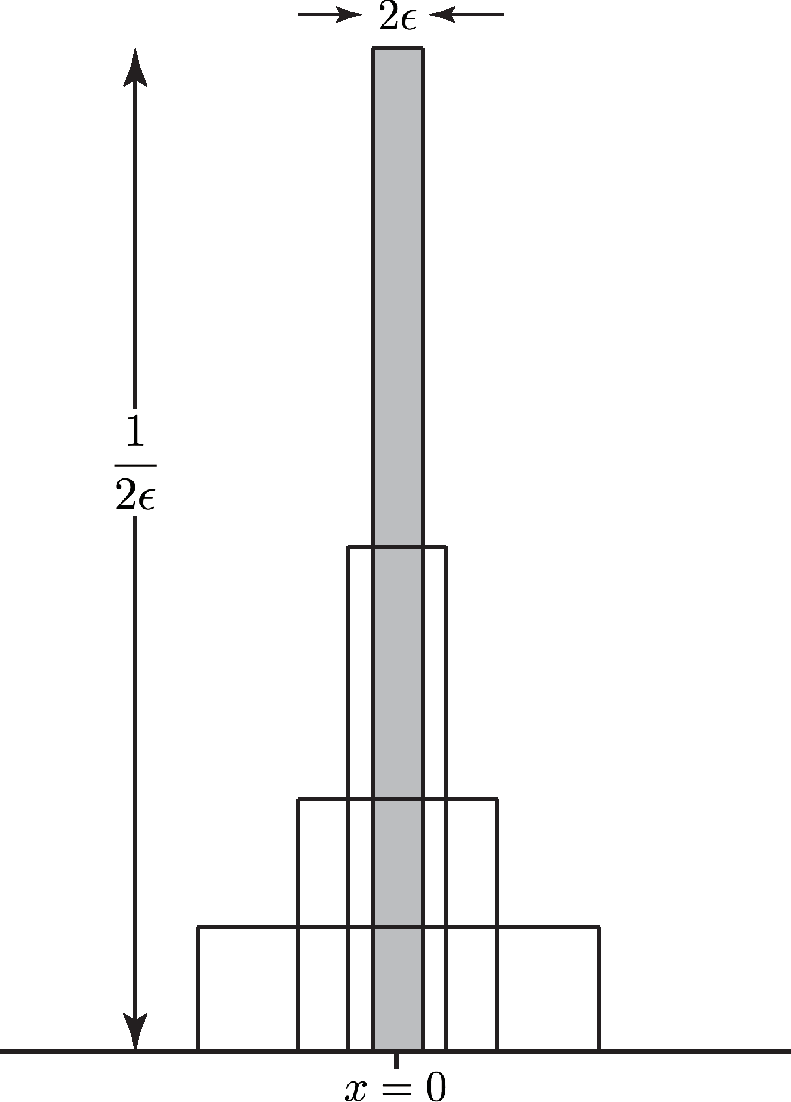
\includegraphics[width=0.5\textwidth]{./Pictures/fig.1.1.pdf}
 \caption{一系列函数递次接近 Dirac delta 函数 $\delta(x)$}
 \label{fg:1.1}
\end{figure}

\exercise{
 应用前面关于 Dirac delta 函数的表述,证明:
 \[a(0) = \int_{-\infty}^\infty \mrm{d}x\,a(x)\delta(x)\]
}

直到现在我们的讨论都与\autoref{sec:1.1.4}中关于$N$维复矢量空间的讨论类似。
确实,完备正交归一函数的理论可以看做普通线性代数的一个推广。
为了方便突显这种相似性,我们引入一种简略表达方式:
\begin{subequations}
 \begin{equation}
     \psi_i(x) \equiv \ket{i} \qquad \psi_i^\ast(x) \equiv \bra{i}
     \label{eq:1.127a}
 \end{equation}
 或更为普遍的:
 \begin{equation}
     a(x) \equiv \ket{a} \qquad a^\ast(x) \equiv \bra{a}
     \label{eq:1.127b}
 \end{equation}
 \label{eq:1.127}
\end{subequations}
以及,两个函数的标量积定义为:
\begin{equation}
 \int \mrm{d}x\,a^\ast(x)b(x) = \olp{a}{b}
 \label{eq:1.128}
\end{equation}
正交归一条件\autoref{eq:1.116}则变为:
\begin{equation}
 \olp{i}{j} = \delta_{ij}
 \label{eq:1.129}
\end{equation}
在这种符号体系下,\autoref{eq:1.118}写作:
\begin{equation}
 \olp{j}{a} = a_j
 \label{eq:1.130}
\end{equation}
因此,\autoref{eq:1.117}变为:
\begin{equation}
 \ket{a} = \sum_i \ket{i}\olp{i}{a}
 \label{eq:1.131}
\end{equation}
需要注意的是,
\autoref{eq:1.129}、\autoref{eq:1.130}和\autoref{eq:1.131}在形式上分别与前一节中的\autoref{eq:1.47}、\autoref{eq:1.48a}和\autoref{eq:1.50a}是完全等同的。

现在我们定义一个算符$\op{O}$,
作用在一个函数$a(x)$上,生成另一个函数$b(x)$:
\begin{subequations}
 \begin{equation}
     \op{O}a(x) = b(x)
     \label{eq:1.132a}
 \end{equation}
 也可以用新引入的符号体系重写为:
 \begin{equation}
     \op{O}\ket{a} = \ket{b}
     \label{eq:1.132b}
 \end{equation}
 \label{eq:1.132}
\end{subequations}
上式与\autoref{eq:1.52}等同。
如果通过需要如下方式计算$b(x)$:
\begin{equation}
 b(x) = \op{O}a(x) = \int\mrm{d}x\,O(x,x^\prime)a(x^\prime)
 \label{eq:1.133}
\end{equation}
则称$\op{O}$为\emph{非定域}算符:
即便我们仅需计算$b(x)$在$x=x_0$处的值,
也需要知道$a(x)$在整个区间上的取值。
非定域算符有时也被称作积分算符。
还需注意,\autoref{eq:1.133}是下式在连续变量情形下的推广:
\begin{equation}
 b_i = \sum_j O_{ij}a_j
 \label{eq:1.134}
\end{equation}
因此,我们可以将$O(x,x^\prime)$看做一个连续矩阵。
如果计算$b(x)$在点$x=x_0$的值时,
只需要知道$a(x)$在$x_0$附近的一个无穷小邻域内的值,
则称$\op{O}$为\emph{定域}算符。
微分算符$\mrm{d}/\mrm{d}x$便是一个定域算符。
如果下面关系成立:
\begin{subequations}
 \begin{equation}
     \op{O}\phi_{\alpha}(x) = \omega_\alpha \phi_\alpha(x)
     \label{eq:1.135a}
 \end{equation}
 或者用 Dirac 符号写为:
 \begin{equation}
     \op{O}\ket{\alpha} = \omega_\alpha\ket{\alpha}
     \label{eq:1.135b}
 \end{equation}
 \label{eq:1.135}
\end{subequations}
与矩阵代数类比,
我们称$\phi_\alpha(x)$为算符$\op{O}$关于本征值$\omega_\alpha$的\emph{本征函数}。
可以选取归一化的函数为本征函数:
\begin{equation}
 \int\mrm{d}x\, \phi_\alpha^\ast(x)\phi_\alpha(x) \equiv \olp{\alpha}{\alpha} = 1
 \label{eq:1.136}
\end{equation}
将\autoref{eq:1.135a}两边乘以$\phi_\alpha^\ast(x)$,
然后对$x$积分,应用\autoref{eq:1.136},
我们得到:
\begin{equation}
 \omega_\alpha = \int \mrm{d}x\,\phi_\alpha^\ast(x)\op{O}\phi_\alpha(x) \equiv \Mele{\alpha}{O}{\alpha}
 \label{eq:1.137}
\end{equation}
此处我们引入了新的符号:
\begin{equation}
 \int\mrm{d}x\,a^\ast(x)\op{O}b(x) = \Mele{a}{O}{b}
 \label{eq:1.138}
\end{equation}
需要注意,我们同样可以在\autoref{eq:1.135b}两边左乘$\bra{a}$,
然后应用归一化条件\eqref{eq:1.136},
得到相同的结果\autoref{eq:1.137}。
此后,我们将把``乘$a^\ast(x)$以然后对$x$积分''简单地表述为``左乘$\bra{a}$''。

与前节相同,
我们同样对 Hermitian算符的本征函数和本征值感兴趣。
Hermitian算符满足如下条件:
\begin{equation}
 \int\mrm{d}x\,a^\ast(x)\op{O}b(x) = \int\mrm{d}x\,b(x)\left(\op{O}a(x)\right)^\ast = \left(\int\mrm{d}x\,b^\ast(x)\op{O}a(x)\right)^\ast
 \label{eq:1.139}
\end{equation}
应用\autoref{eq:1.138}引入的符号,上式可写为:
\begin{equation}
 \Mele{a}{O}{b} = {\Mele{b}{O}{a}}^\ast
 \label{eq:1.140}
\end{equation}
注意上式与\autoref{eq:1.61}具有相同的形式。
Dirac 符号的优美之处在于,它允许我们用完全相同的形式来处理矢量和函数,
以及作用于它们的算符。
比如,\autoref{sec:1.1.6}中关于 Hermitian算符的本征值和本征矢性质的证明,
可以直接应用于 Hermitian算符的本征值和本征函数上。
因此,Hermitian算符的本征函数是正交归一的,
它们对应的本征值为实数。

\exercise{
 为了进一步展示我们所采用的符号体系的自洽性,
 考虑算符$\op{O}$在基组$\left\{\psi_i(x)\right\}$中的矩阵表示:
 已知
 \[\op{O}\psi_i(x) = \sum_j\psi_j(x)O_{ji}\]
 证明
 \[O_{ji} = \int\mrm{d}x\,\psi_j^\ast(x)\op{O}\psi_i(x)\]
 然后应用\autoref{eq:1.127a}和\autoref{eq:1.138},
 用 Dirac 符号重写第一个方程,
 并证明其与\autoref{eq:1.55}等价。
\Next
 考虑如下本征值问题:
 \[\op{O}\phi(x) = \omega\phi(x)\]
 通过将$\phi$在完备基组$\left\{\psi_i(x),\, i = 1, 2, \dots\right\}$ 中展开:
 \[\phi(x) = \sum_i^\infty c_i \psi_i(x)\]
 证明等价于矩阵的本征值问题:
 \[\mbf{O}\mbf{c} = \omega\mbf{c}\]
 此处,$(\mbf{c}_i) = c_i$,$(\mbf{O})_{ij} = \int\mrm{d}x \psi_i^\ast(x) \op{O} \psi_j(x)$。
 分别用普通形式和 Dirac 符号完成以上证明。
 需要注意的是,此处$\mbf{O}$是一个无穷矩阵,
 而实际操作中,我们无法处理无穷矩阵。
 为了使问题可操作,
 我们可以选取无穷基组的一个子集$\left\{\psi_i(x),\, i = 1, 2, \dots, N\right\}$。
 如果在这个子空间中重复以上分析,
 我们会得到一个$N\times N$维的本征值问题。
 我们将在\autoref{sec:1.3}中看到,
 此处得到的$N$个本征值是真实本征值的近似。
 重要的是,
 我们需要证明这个截断的本征值问题的最低本征值不低于真实的最低本征值。
\Next

 本小节中我们使用了Dirac符号体系的简化版本,
 这种简化相对于我们的目的来说够用,
 但对矢量和函数之间的密切关系描述过于简单。
 在这个练习中,我们将初步感受一下 Dirac 符号体系的强大之处。
 考虑一个由完备正交归一基矢构成的可数无限集,即:
\[
     \sum_i^\infty \ket{i}\bra{a} = 1
     \tag{1a}\label{eq:e1.17.1a}
\]
\[
     \olp{i}{j} = \delta_{ij}
     \tag{1b}\label{eq:e1.17.1b}
\]
引入连续变量的无限完备基组,
其基组为$\ket{x}$。与\autoref{eq:e1.17.1a}类似:
\[
\int\mrm{d}x\,\ket{x}\bra{x} = 1
\tag{2a}\label{eq:e1.17.2a}
\]
在上式中,我们将\autoref{eq:e1.17.1a}中的加和替换成了积分。
将\autoref{eq:e1.17.2a}两边左乘$\bra{a}$,右乘$\ket{b}$,我们有:
\[
\int\mrm{d}x\, \olp{a}{x}\olp{x}{b} = \olp{a}{b}
\]
与\autoref{eq:1.128}相比,
我们可以认出,
$\olp{a}{x}$即$a^\ast(x)$,$\olp{x}{b}$即$b(x)$。
我们知道$\olp{i}{a}$是$\ket{a}$沿基矢$\ket{i}$的分量。
因此,
我们可以将函数$b(x)$看做是抽象矢量$\ket{b}$在一个具有连续变量的无限多坐标轴的坐标系中沿$x$的分量。
\begin{enumerate}[a.]
 \item 将\autoref{eq:e1.17.2a}两边左乘$\bra{i}$,右乘$\ket{j}$,应用\autoref{eq:e1.17.1b},证明若有如下关系成立:
 \[
 \psi^\ast_i(x) = \olp{i}{x} \qquad \psi_j(x) = \olp{x}{j}
 \]
 则所得结果与\autoref{eq:1.116}等同。
 \item 将\autoref{eq:e1.17.1a}两边左乘$\bra{x}$,右乘$\ket{x^\prime}$。证明若有如下关系成立
 \[
 \olp{x}{x^\prime} = \delta(x - x^\prime)
 \tag{2b} \label{eq:e1.17.2b}
 \]
 则所得结果与\autoref{eq:1.120}等同。上式即为\autoref{eq:e1.17.1b}在连续变量情形下的类比。
 \item 将\autoref{eq:e1.17.2a}两边左乘$\bra{x^\prime}$,右乘$\ket{a}$。证明所得方程与\autoref{eq:1.121}等同。
 \item 一个算符$\op{O}$在连续基$\ket{x}$中的矩阵表示为
 \[\Mele{x}{O}{x^\prime} = O(x, x^\prime)\]
 由式$\op{O}\ket{a} = \ket{b}$出发并插入完备性关系,我们有
 \[\op{O}\ket{a} = \op{O}\mbf{1}\ket{a} = \int\mrm{d}x\,\op{O}\ket{x}\bra{x}\ket{a} = \ket{b}\]
 将上式左乘$\bra{x^\prime}$,验证结果与\autoref{eq:1.133}等同。
 \item 若有$O_{ij} = \Mele{i}{O}{j}$,验证:
 \[O(x,x^\prime) = \sum_{ij}\psi_i(x)O_{ij}\psi_j^\ast(x)\]
\end{enumerate}
}


\section{变分法}
\label{sec:1.3}
本节讨论近似求解本征值问题的一种重要方法。本征值问题即:
\begin{equation}
 \op{O}\psi(x) =\omega\psi(x)
 \label{eq:1.141}
\end{equation}
我们对此感兴趣是因为不含时的(定态) Schr\"{o}dinger 就是一个本征方程:
\begin{equation}
 \op{H} \ket{\Phi} = \mcr{E} \ket{\Phi}
 \label{eq:1.142}
\end{equation}
其中,$\op{H}$为 Hamiltonian,是一个 Hermitian算符,
$\ket{\Phi}$是波函数,$\op{E}$是体系能量。
除了最简单的体系,无法对Schr\"odinger 方程精确求解,
因此,我们关心如何求得这个本征值问题的近似解。
虽然接下来的内容可以应用于任意的特征值问题,
但是我们将沿用 Schr\"odinger 方程\autoref{eq:1.142}相关的符号和术语。

给定算符$\op{H}$,存在一个 Schr\"odinger 方程的精确解的无限集合,我们用$\alpha$来标记:
\begin{equation}
 \op{H}\ket{\Phi_\alpha} = \op{E}_\alpha\ket{\Phi_\alpha}
 \label{eq:1.143}
\end{equation}
其中
\[
\op{E}_0 \leq \op{E}_1 \leq \op{E}_2 \leq \cdots \leq \op{E}_\alpha \leq \cdots
\]
简便起见,
此处我们假设本征值的集合$\left\{\op{E}_\alpha\right\}$是离散的。
由于$\op{H}$是 Hermitian算符,
其本征值$\mcr{E}_\alpha$是实数,
且其对应的本征函数是正交归一的:
\begin{equation}
 \olp{\Phi_\alpha}{\Phi_\beta} = \delta_{\alpha\beta}
 \label{eq:1.144}
\end{equation}
\autoref{eq:1.143}两边左乘$\bra{\Phi_\beta}$得到:
\begin{equation}
 \Mele{\Phi_\beta}{H}{\Phi_\alpha} = \mcr{E}_\alpha\delta{\alpha\beta}
 \label{eq:1.145}
\end{equation}
此外,我们还假设$\op{H}$的本征函数构成一个完备基,
因此,任意一个与$\left\{\ket{\Phi_\alpha}\right\}$具有相同的边界条件的函数$\vert\tilde{\Phi}\rangle$,都可以写为$\ket{\Phi_\alpha}$的线性组合:
\begin{equation}
 \Ket{\tilde{\Phi}} = \sum_\alpha \mathinner{\Big\vert\Phi_\alpha\Big\rangle} c_\alpha = \sum_\alpha \Big\vert\Phi_\alpha\Big\rangle \Olp{\Phi_\alpha}{\tilde{\Phi}}
 \label{eq:1.146}
\end{equation}
以及
\begin{equation}
 \Bra{\tilde\Phi} = \sum_\alpha c_\alpha^\ast \Big\langle\Phi_\alpha\Big\vert = \sum_\alpha \Olp{\tilde\Phi}{\Phi_\alpha}\Big\langle\Phi_\alpha\Big\vert
 \label{eq:1.147}
\end{equation}

\subsection{变分原理}
\label{sec:1.3.1}
现在我们给出一个重要的定理,即\emph{变分原理},的描述,并给予证明:
对于一个符合恰当边界条件(通常是在无穷远处波函数为零)的归一化的波函数$\ket{\tilde\Phi}$,
其 Hamiltonian 的期望值是精确基态能量的上限。即,若有
\begin{equation}
 \Big\langle\tilde\Phi\Big\vert\tilde\Phi\Big\rangle = 1
 \label{eq:1.148}
\end{equation}
则
\begin{equation}
 \Big\langle\tilde\Phi\Big\vert\op{H}\Big\vert\tilde\Phi\Big\rangle \geq \mcr{E}_0
 \label{eq:1.149}
\end{equation}
此定理的证明比较简单
\footnote{
译注:此处原书的证明有些冗余,实际上证明变分定理无需第二套基底$\Ket{\Phi_\beta}$。考虑
\[
    \Olp{\tilde\Phi}{\tilde\Phi} = \sum_\alpha \Big\langle\tilde\Phi\Big\vert\Phi_\alpha\Big\rangle\Big\langle\Phi_\alpha\Big\vert\tilde\Phi\Big\rangle = \sum_\alpha \Big\vert\Big\langle\Phi_\alpha\Big\vert\tilde\Phi\Big\rangle\Big\vert^2 = 1
\]
上式用到了\autoref{eq:1.146}。然后,
\[
    \Langle\tilde\Phi\Lvert\op{H}\Lvert\tilde\Phi\Rangle =  \sum_\alpha \mcr{E}_\alpha \Lvert\Langle\Phi_\alpha\Lvert\tilde\Phi\Rangle\Lvert^2
\]
上式用到了\autoref{eq:1.143}。最后,对于所有$\alpha$有$\mcr{E}_\alpha \geq \mcr{E}_0$,我们得到
\[
    \Langle\tilde\Phi\Lvert\op{H}\Lvert\tilde\Phi\Rangle = \sum_\alpha \mcr{E}_\alpha\Lvert\Langle\Phi_\alpha\Lvert\tilde\Phi\Rangle\Lvert^2 \geq \sum_\alpha \mcr{E}_0\Lvert\Langle\Phi_\alpha\Lvert\tilde\Phi\Rangle\Lvert^2 = \mcr{E}_0\sum_\alpha \Lvert\Langle\Phi_\alpha\Lvert\tilde\Phi\Rangle\Lvert^2 = \mcr{E}_0
\]
即可证明\autoref{eq:1.149},即变分原理。
}
。首先我们考虑
\begin{equation}
 \begin{split}
     \Olp{\tilde\Phi}{\tilde\Phi} &= 1 = \sum_{\alpha\beta}\Big\langle\tilde\Phi\Big\vert\Phi_\alpha\Big\rangle\Big\langle\Phi_\alpha\Big\vert\Phi_\beta\Big\rangle\Big\langle\Phi_\beta\Big\vert\tilde\Phi\Big\rangle = \sum_{\alpha\beta} \Big\langle\tilde\Phi\Big\vert\Phi_\alpha\Big\rangle\delta_{\alpha\beta}\Big\langle\Phi_\beta\Big\vert\tilde\Phi\Big\rangle \\
     &= \sum_\alpha \Big\langle\tilde\Phi\Big\vert\Phi_\alpha\Big\rangle\Big\langle\Phi_\alpha\Big\vert\tilde\Phi\Big\rangle = \sum_\alpha \Big\vert\Big\langle\Phi_\alpha\Big\vert\tilde\Phi\Big\rangle\Big\vert^2
 \end{split}
 \label{eq:1.150}
\end{equation}
其中,我们用到了\autoref{eq:1.144}、\autoref{eq:1.146}和\autoref{eq:1.147}。然后,
\begin{equation}
 \Langle\tilde\Phi\Lvert\op{H}\Lvert\tilde\Phi\Rangle = \sum_{\alpha\beta}\Langle\tilde\Phi\Lvert\Phi_\alpha\Rangle\Langle\Phi_\alpha\Lvert\op{H}\Lvert\Phi_\beta\Rangle\Langle\Phi_\beta\Lvert\tilde\Phi\Rangle = \sum_\alpha \mcr{E}_\alpha \Lvert\Langle\Phi_\alpha\Lvert\tilde\Phi\Rangle\Lvert^2
 \label{eq:1.151}
\end{equation}
上式用到了\autoref{eq:1.145}。最后,由于对于所有$\alpha$有$\mcr{E}_\alpha \geq \mcr{E}_0$,我们得到
\begin{equation}
 \Langle\tilde\Phi\Lvert\op{H}\Lvert\tilde\Phi\Rangle \geq \sum_\alpha \mcr{E}_0\Lvert\Langle\Phi_\alpha\Lvert\tilde\Phi\Rangle\Lvert^2 = \mcr{E}_0\sum_\alpha \Lvert\Langle\Phi_\alpha\Lvert\tilde\Phi\Rangle\Lvert^2 = \mcr{E}_0
 \label{eq:1.152}
\end{equation}
此处我们用到了正交化条件\autoref{eq:1.150}。

关于基态的变分原理告诉我们,
近似波函数的能量总是过高。
因此,可以用期望能量来检测波函数的质量:
能量越低,波函数质量越好。
上述即为变分原理的基础:
我们采用了一个归一化的试探函数$\ket{\tilde\Phi}$,
这个试探函数具有某些参数,
改变这些参数使得期望值$\Mele{\tilde\Phi}{H}{\tilde\Phi}$达到其极小值。
这个极小值就是精确基态能量的变分估值。

\exercise{
 原子单位下,在势场$-\delta(x)$中进行一维运动的电子的 Schr\"odinger 方程为:
 \[
 \left(-\frac{1}{2}\frac{\mrm{d}^2}{\mrm{d}x^2} - \delta(x)\right) \ket{\Phi} = \mcr{E}\ket{\Phi}
 \]
 采用如下试探函数,
 \[\Lvert\tilde\Phi\Rangle = N \mrm{e}^{-\alpha x^2}\]
 应用变分法,验证$-\pi^{-1}$是精确基态能量(-0.5)的一个上限。
 计算中可能会用到如下积分:
 \[
 \int_{-\infty}^{\infty}\mrm{d}x\,x^{2m}\mrm{e}^{-\alpha x^2} = \frac{(2m)!\,\pi^{1/2}}{2^{2m}m!\,\alpha^{m+1/2}}
 \]
\Next
 原子单位下,氢原子的 Schr\"odinger 方程为:
 \[
 \left(-\frac{1}{2}\nabla^2 - \frac{1}{r}\right)\ket{\Phi} = \mcr{E}\ket\Phi
 \]
 应用变分法并采用如下试探函数:
 \[
 \Ket{\tilde{\Phi}} = N \mrm{e}^{-\alpha r^2}
 \]
 验证$-4/3\pi = -0.4244$是精确基态能量(-0.5)的一个上限。
 计算中可能会用到如下公式:
 \[
 \nabla^2f(r) = r^{-2}\frac{\mrm d}{\mrm{d}r}\left(r^2\frac{\mrm d}{\mrm{d}r}\right)f(r)
 \]
 \[
 \int_0^\infty \mrm{d}r\, r^{2m}\mrm{e}^{-\alpha r^2} = \frac{(2m)!\,\pi^{1/2}}{2^{2m+1}m!\,\alpha^{m+1/2}}
 \]
 \[
 \int_0^\infty\mrm{d}r\,r^{2m+1}\mrm{e}^{-\alpha r^2} = \frac{m!}{2\alpha^{m+1}}
 \]
\Next
 将变分原理应用于矩阵本征值问题时用到的列矢量$\mbf{c}$是归一化的($\madj{c}\mbf{c} = 1$),
 由此我们得到$\madj{c}\mbf{Oc}$不低于矩阵$\mbf{O}$的最低本征值的结论。
 对于一个$2\times2$对称矩阵($O_{12}=O_{21}$),
 \[ \mbf{O} = 
 \begin{pmatrix}
     O_{11} & O_{12} \\ O_{21} & O_{22}
 \end{pmatrix}
 \]
 采用归一化的试探矢量
 \[ \mbf{c} = \begin{pmatrix}
     \cos\theta \\ \sin\theta
 \end{pmatrix}
 \]
 计算
 \[\omega(\theta) = \madj{c}\mbf{O}\mbf{c}\]
 并指出使$\omega(\theta)$取极小值的$\theta$,
 即$\theta_0$。
 验证$\omega(\theta_0)$与矩阵$\mbf O$的最低本征值(见\autoref{eq:1.105} 和\autoref{eq:1.106a}相等。
 你对这个结果有什么想法?
}


\subsection{线性变分问题}
\label{sec:1.3.2}
若试探函数$\ket{\tilde\Phi}$包含一系列参数,
则其期望值$\langle\tilde\Phi\vert\op{H}\vert\tilde\Phi\rangle$也取决于这些参数。
通常情况下,
寻找使$\langle\tilde\Phi\vert\op{H}\vert\tilde\Phi\rangle$取极小值的那组参数的值是一个非常复杂的问题,
以至于没有简单的方法来完成。
然而,如果我们只允许试探函数存在线性的变化,即:
\begin{equation}
 \Ket{\tilde\Phi} = \sum_{i=1}^{N} c_i \Lvert\Psi_i\Rangle
 \label{eq:1.153}
\end{equation}
其中,$\left\{\vert\Psi_i\rangle\right\}$是一组\emph{固定}的基函数,
这样我们将问题转变成寻找最优化的系数$\left\{c_i\right\}$将矩阵对角化。

假设我们的基函数是实函数,并满足正交归一条件
\begin{equation}
 \left\langle\Psi_i\middle\vert\Psi_j\right\rangle = \left\langle\Psi_j\middle\vert\Psi_i\right\rangle = \delta_{ij}
 \label{eq:1.154}
\end{equation}
非正交归一的复函数的情形我们将在\autoref{ch:3}中讨论。
Hamiltonian 算符在基组$\left\{\vert\Psi_i\rangle\right\}$中的矩阵表示$\mbf{H}$是一个$N\times N$的矩阵,
其矩阵元为:
\begin{equation}
 \left(\mbf{H}\right)_{ij} = H_{ij} = \Mele{\Psi_i}{H}{\Psi_j}
 \label{eq:1.155}
\end{equation}
由于 Hamiltonian 是 Hermitian,且
基函数为实函数,$\mbf H$为对称矩阵,
即$H_{ij} = H_{ji}$。试探函数满足归一化条件
\begin{equation}
 \Olp{\tilde\Phi}{\tilde\Phi} = \sum_{ij} c_i c_j \Langle\Psi_i\Lvert\Psi_j\Rangle = \sum_i c_i^2 = 1
 \label{eq:1.156}
\end{equation}
其期望值
\begin{equation}
 \Mele{\tilde\Phi}{H}{\tilde\Phi} = \sum_{ij}c_i\Langle\Psi_i\Lvert\op{H}\Lvert\Psi_j\Rangle c_j = \sum_{ij}c_ic_jH_{ij}
 \label{eq:1.157}
\end{equation}
是关于展开系数的函数。

我们的问题是寻找使$\langle\tilde\Phi\vert\op{H}\vert\tilde\Phi\rangle$取极小值的那组参数。
不幸的是,这$N$个参数不是互相独立的,
因此我们不能简单地求解如下方程:
\begin{equation}
 \frac{\partial}{\partial c_k} \Mele{\tilde\Phi}{H}{\tilde\Phi} = 0 \qquad k = 1, 2, \dots, N
 \label{eq:1.158}
\end{equation}
由于试探函数是归一化的,
展开系数之间的关系满足\autoref{eq:1.158},
即只有$N-1$个独立变量。
在约束条件(\autoref{eq:1.156})下将函数~\eqref{eq:1.157}最小化的问题可以用 Lagrange \emph{不定乘子法}来解决:首先构建一个函数

\begin{equation}
 \begin{split}
     \mcr{L}\left(c_1, \dots, c_N, E\right) &= \Mele{\tilde\Phi}{H}{\tilde\Phi} - E\left(\Olp{\tilde\Phi}{\tilde\Phi} - 1\right) \\
     &= \sum_{ij} c_ic_jH_{ij} - E\left(\sum_i c_i^2 -1\right)
 \end{split}
 \label{eq:1.159}
\end{equation}
由于试探函数是归一化的,
实际上我们只在\autoref{eq:1.157}上加了一个零项,
因此函数$\mele{\tilde\Phi}{H}{\tilde\Phi}$ 和$\mcr{L}$在取同一组参数值时同事具有极小值。
如果将$c_1, c_2, \dots, c_{N-1}$选为任意的独立变量,
则$c_N$可以通过归一性条件\autoref{eq:1.156}确定。
这时我们有:
\begin{equation}
 \frac{\partial \mcr{L}}{\partial c_k} = 0 \qquad k = 1, 2, \dots, N-1
 \label{eq:1.160}
\end{equation}
上式并不要求$\partial\mcr{L}/\partial{c_k}$必须为零。
然而,在我们目前的处理过程中还有一个未定乘子$E$,
我们可以选取$E$使得$\partial\mcr{L}/\partial{c_k}$值为零,则有
\begin{equation}
 \frac{\partial \mcr{L}}{\partial c_k} = 0 \qquad k = 1, 2, \dots, N
 \label{eq:1.161}
\end{equation}
因此,
\begin{equation}
 \frac{\partial \mcr{L}}{\partial c_k} = 0 = \sum_j c_j H_{kj} + \sum_i c_i H_{ik} - 2 E c_k
 \label{eq:1.162}
\end{equation}
又因为 $H_{ij} = H_{ji}$,我们有:
\begin{equation}
 \sum_j H_{ij}c_j - Ec_i = 0
 \label{eq:1.163}
\end{equation}
引入列向量$\mbf c$,其元素为$c_i$,则上式可以写为矩阵式:
\begin{equation}
 \mbf{H}\mbf{c} = E \mbf{c}
 \label{eq:1.164}
\end{equation}
即一个标准的关于矩阵$\mbf{H}$的本征值问题。

由于$\mbf{H}$是对称矩阵,
求解\autoref{eq:1.164}将得到$N$个正交归一的本征矢$\mbf{c}^\alpha$及其对应的本征值$E_\alpha$。
方便起见,我们将本征值按照升序排列,
即$E_0 \leq E_1 \leq \cdots \leq E_{N-1}$。因此,
\begin{equation}
 \mbf{H}\mbf{c}^\alpha = E_\alpha \mbf{c}^\alpha\qquad \alpha = 0, 1, \dots, N-1
 \label{eq:1.165}
\end{equation}
其中,
\begin{equation}
 \left(\mbf{c}^\alpha\right)^\dagger\mbf{c}^\beta = \sum_i c_i^\alpha c_i^\beta = \delta_{\alpha\beta}
 \label{eq:1.166}
\end{equation}
我们还可以引入对角矩阵$\mbf{E}$,
其对角元为前述本征值$E_\alpha$,
即$\left(\mbf{E}\right)_\alpha\beta = E_\alpha\delta_{\alpha\beta}$,
以及由本征矢组成的矩阵$\mbf{C}$,
其中$C_{i\alpha} = c_i^\alpha$,
则\autoref{eq:1.165}包含的$N$个关系可以写作:
\begin{equation}
 \mbf{H}\mbf{C} = \mbf{C}\mbf{E}
 \label{eq:1.167}
\end{equation}

通过上述变换,
我们实际上能够同时求出关于$\ket{\tilde\Phi}$的$N$组而不是一组展开系数:
\begin{equation}
 \Ket{\tilde\Phi} = \sum_{i=1}^N c_i^\alpha \Lvert\Psi_i\Rangle = \sum_{i=1}^N C_{i\alpha}\Lvert\Psi_i\Rangle \qquad \alpha = 0, 1, \dots, N-1
 \label{eq:1.168}
\end{equation}
并且这些本征矢满足正交归一关系:
\begin{equation}
 \Langle\tilde\Phi_\alpha\Lvert\tilde\Phi_\beta\Rangle = \sum_{ij} c_i^\alpha c_j^\beta \Langle\Psi_i\Lvert\Psi_j\Rangle = \sum_{ij}c_i^\alpha c_j^\beta\delta_{ij} = \sum_i c_i^\alpha c_i^\beta = \delta_{\alpha\beta}
 \label{eq:1.169}
\end{equation}
上式推导过程中我们用到了\autoref{eq:1.154}和\autoref{eq:1.166}。
我们还需要发掘一下$E$的物理意义,考虑到:
\begin{equation}
 \begin{split}
     \Langle\tilde\Phi_\beta\Lvert\op{H}\Lvert\tilde\Phi_\alpha\Rangle &= \sum_{ij} c_i^\beta \Langle \Psi_i\Lvert\op{H}\Lvert\Psi_j\Rangle c_j^\alpha \\
     &= \sum_{ij}c_j^\beta H_{ij}c_j^\alpha \\
     &= \left(\mbf{c}^\beta\right)^\dagger\mbf{H}\mbf{c}^\alpha \\
     &= E_\alpha \left(\mbf{c}^\beta\right)^\dagger\mbf{c}^\alpha = E_\alpha \delta_{\alpha\beta}
 \end{split}
 \label{eq:1.170}
\end{equation}
此处我们用到了\autoref{eq:1.165}和\autoref{eq:1.166}。
因此,Hamiltonian 的本征值$E_\alpha$就是 对应于$\ket{\tilde\Phi}$的期望值。
特别的,在基函数$\left\{\vert\Psi_i\rangle\right\}$张开的空间中,
最低本征值$E_0$是$\op{H}$的基态能量的最好近似。
此外,变分原理还保证了
\begin{equation}
 E_0 = \Langle\tilde\Phi_0\Lvert\op{H}\Lvert\tilde\Phi_0\Rangle \geq \mcr{E}_0
 \label{eq:1.171}
\end{equation}
那么其他本征值$E$有什么物理意义呢?
可以证明(见\autoref{ex:1.21})
$E_\alpha \geq \mcr{E}_\alpha,\, \alpha = 1, 2, \dots$,因此,$E_1$是第一激发态能量的上限,以此类推。

\exercise{
          考虑一个归一化的试探函数$\ket{\tilde\Phi^\prime}$,
          其正交于精确的基态波函数,即$\langle \tilde \Phi^\prime \vert \Phi_0 \rangle = 0$
 \begin{enumerate}[a.]
     \item 推广\autoref{sec:1.3.1}中关于变分原理的证明,并验证
     \[\Langle\tilde{\Phi}^\prime\Lvert\op{H}\Lvert\tilde{\Phi}^\prime\Rangle \geq \mcr{E}_1.\]
     \item 考虑如下函数
     \[\Lvert\tilde{\Phi}^\prime\Rangle = x\Lvert\tilde\Phi_0\Rangle + y \Lvert\tilde\Phi_1\Rangle\]
     其中$\ket{\tilde\Phi_\alpha}, \alpha = 0, 1$由\autoref{eq:1.168}给定。
     若该函数归一,证明
     \[\vert x\vert^2 + \vert y \vert^2 = 1.\]
     \item 若选定$x$和$y$使得$\ket{\tilde\Phi^\prime}$归一,
     且满足关系$\olp{\tilde\Phi^\prime}{\Phi_0} = 0$,
     则可由 (a) 得出$\mele{\tilde\Phi^\prime}{H}{\tilde\Phi^\prime} \geq \mcr{E}_1$。
     验证如下关系:
     \[\Mele{\tilde\Phi^\prime}{H}{\tilde\Phi^\prime} = E_1 - \vert x\vert^2 (E_1 - E_0) \]
     由于$E_1 \geq E_0$,我们可以得到结论$E_1 \geq \Mele{\tilde\Phi^\prime}{H}{\tilde\Phi^\prime} \geq \mcr{E}_1$。推广以上论证,证明$E_\alpha \geq \mcr{E}_\alpha,\, \alpha = 2, 3, \dots .$
 \end{enumerate}
}

总之,线性变分法是在给定一组固定的正交归一函数$\left\{\ket{\Psi_i},\,i=1, 2, \dots, N\right\}$的情况下,
为本征值问题
\begin{equation}
 \op{H}\Ket{\Phi} = \mcr{E}\Ket{\Phi}
 \label{eq:1.172}
\end{equation}
寻找最优近似解的一种方法。
该方法需要在有限基组$\left\{\ket{\Psi_i}\right\}$内构建算符$\op{H}$的矩阵表示,
即$(\mbf{H})_{ij} = \mele{\Psi_i}{H}{\Psi_j}$,
并求解矩阵本征值问题:
\begin{equation}
 \mbf{H}\mbf{c} = E \mbf{c}
 \label{eq:1.173}
\end{equation}
即将$N\times N$矩阵$\mbf H$对角化。

前面我们通过直接对 Hamiltoninan 的期望值求极小值得到上述结论。
然而,还可以通过其他方法来得到\autoref{eq:1.173},
我们将发现这种方法另有助益:
在求解\autoref{eq:1.172}时,假设
\begin{equation}
 \Ket{\Phi} = \sum_{j=1}^N c_j\Ket{\Psi_j}
 \label{eq:1.174}
\end{equation}
将上式带入\autoref{eq:1.172}:
\begin{equation}
 \sum_j c_j \op{H}\Ket{\Psi_j} = \mcr{E} \sum_j c_j \Ket{\Psi_j}
 \label{eq:1.175}
\end{equation}
上式两边左乘$\bra{\Psi_i}$,由于展开\autoref{eq:1.174}为近似式,将$\mcr{E}$替换为$E$,则有:
\[
\sum_j c_j \Mele{\Psi_i}{H}{\Psi_j} = E\sum_j c_j \Olp{\Psi_i}{\Psi_j} = Ec_i
\]
或写为:
\begin{equation}
 \sum_j H_{ij}c_j = E c_i
 \label{eq:1.176}
\end{equation}
上式的矩阵式与\autoref{eq:1.173}等同。
如果使用\emph{完备}的正交归一基组 $\left\{\ket{\Psi_i},
\right. \, i = 1, 2,\allowbreak \dots, N, N+1, \left.\dots \right\}$,
我们则会得到一个与\autoref{eq:1.173}等同,
但其中的$\mbf{H}$为一个无限矩阵。
在这种情况下,矩阵的本征值会与算符$\op{H}$的本征值严格相等。
因此,线性变分法就相当于在由基函数$\left\{\ket{\Psi_i},\,i=1,2,\dots,N\right\}$张开的有限子空间中求解本征值问题\autoref{eq:1.172}。
 
\exercise{
     原子单位下,处于一个指向$z$向的场强为$F$的匀强电场中的氢原子的 Schr\"odinger 方程为:
 \[
 \left(-\frac{1}{2}\nabla^2 - \frac{1}{r} + Fr\cos\theta\right) \Ket{\Phi} = \left(\op{H}_0 + Fr\cos\theta\right)\Ket{\Phi} = \mcr{E}(F)\Ket{\Phi}
 \]
 使用如下试探函数,求$\mcr{E}(F)$的上限。
 \[\Ket{\tilde{\Phi}} = c_1\Lvert 1s\Rangle + c_2 \Lvert 2p_z\Rangle\]
 其中$\ket{1s}$和$\ket{2p_z}$是$\op{H}$的正交归一本征函数,即:
 \[
 \begin{split}
     \Ket{1s} &= \pi^{-1/2}\mrm{e}^{-r} \\
     \Ket{2p_z} &= (32\pi)^{-1/2}r\mrm{e}^{-r/2}\cos\theta
 \end{split}
 \]
 在构建$\op{H}$的矩阵表示时,可以使用如下关系:
 \[
 \op{H}_0 \Ket{1s} = -\frac{1}{2}\Ket{1s},\qquad \op{H}_0 \Ket{2p_z} = -\frac{1}{8}\Ket{2p_z}
 \]
 利用公式$(1+x)^{1/2} \approx 1 + x/2$,将所得结果对$F$进行 Taylor 展开,即:
 \[
 E(F) = E(0) -\frac{1}{2}\alpha F^2 + \cdots
 \]
 其中$\alpha$为体系近似的偶极极化率,验证其值为 2.96。其精确结果为 4.5。
}
 
\addcontentsline{toc}{section}{\protect\numberline{}{扩展阅读}}
 
\begin{description}
 \item{Acton, F. S., \textit{Numerical Methods that Work}, Harper \& Row, New York, 1970.} 该书第13章有关于矩阵本征值问题的各种高效算法的非常好的讨论。
 \item{Cushing, J. T. \textit{Applied Analytical Mathematics for Physical Scientists}, Wiley, New York, 1975.} 该书的前四章对本章中的数学进行了一个严格但易接受的讲述。
 \item{Merzbacher, E., \textit{Quantum Mechanics}, 2nd ed., Wiley, New York, 1970.} 多数研究生用的量子力学教材都完整讲授了 Dirac 符号。该书的第 14 章包含这部分内容的一个导论。
 \item{Press, W. H., Flannery, B. P., Teukolsky, S. A. and Vetterling, W. T. \textit{Numerical Recipes}, Cambridge University Press, Cambridge, 1986.} 在这部科学计算的圣经中,第11章讨论了寻找矩阵本征值和本征矢的多种算法,并提供了 FORTRAN 源码。
\end{description}